% Load the kaobook class
\documentclass[
	fontsize=10pt, % Base font size
	twoside=false, % Use different layouts for even and odd pages (in particular, if twoside=true, the margin column will be always on the outside)
	%open=any, % If twoside=true, uncomment this to force new chapters to start on any page, not only on right (odd) pages
	secnumdepth=2, % How deep to number headings. Defaults to 1 (sections)
	numbers=noenddot,
]{kaobook}

% Choose the language
\usepackage[english]{babel} % Load characters and hyphenation
\usepackage[english=british]{csquotes}	% English quotes

% TODO notes
\usepackage{todonotes}

% Change format of vectors to boldface without arrow.
\usepackage{bm}
\renewcommand\vec{\mathbf}

% Load packages for testing
\usepackage{blindtext}
%\usepackage{showframe} % Uncomment to show boxes around the text area, margin, header and footer
%\usepackage{showlabels} % Uncomment to output the content of \label commands to the document where they are used

% Load the bibliography package
\usepackage{kaobiblio}
\addbibresource{library.bib} % Bibliography file

% Load mathematical packages for theorems and related environments
\usepackage{kaotheorems}

% Load the package for hyperreferences
\usepackage{kaorefs}

% To be able to include Tikz files
% \usepackage{standalone}

% To typeset date and time
\usepackage{datetime2}
\DTMsetstyle{ddmmyyyy}

% For logos on titlepage.
\usepackage{tabularx}

% To typeset units
\usepackage[separate-uncertainty=true]{siunitx}
\DeclareSIUnit\stretch{unit\,stretch}

% To rotate big images sideways
\usepackage{rotating}
% \usepackage{pdflscape}

% To display svg images.
\usepackage[inkscapelatex=false]{svg}
% \newcommand{\kutblokje}[1]{%
% 	\begin{tikzpicture}
	
% 		\node[rectangle,draw] (r) at (0,0) {};
	
% 	\end{tikzpicture}
% }
% \DeclareUnicodeCharacter{25AF}{\kutblokje{}}

% \newcommand{\ie}{i.\,e.\,}
% \newcommand{\Ie}{I.\,e.\,}
% \newcommand{\eg}{e.\,g.\,}
% \newcommand{\Eg}{E.\,g.\,}

% For logos on title page
\newcolumntype{u}{>{\hsize=0.56\hsize}X}
\newcolumntype{v}{>{\hsize=0.44\hsize}X}

% For check/x-marks
\usepackage{pifont}% http://ctan.org/pkg/pifont
\newcommand{\cmark}{\ding{51}}%
\newcommand{\xmark}{\ding{55}}%

\usepackage{fontawesome5}

% For iterating on images in a directory, using foreach.
\usepackage{pgffor}%

\graphicspath{{images/}{./}} % Paths where images are looked for

\makeindex[columns=3, title=Alphabetical Index, intoc] % Make LaTeX produce the files required to compile the index

% https://github.com/fmarotta/kaobook/issues/145#issuecomment-866744813
% \makeatletter
% \RenewDocumentCommand{\chapterstylekao}{}{%
%     \renewcommand*{\chapterformat}{%
%         \mbox{\chapappifchapterprefix{\nobreakspace}\scalebox{2.85}{\thechapter\autodot}}%
%     }%  
%     \renewcommand\chapterlinesformat[3]{%
%         \vspace{3.5\vscale}%
%         \if@twoside%
%             \Ifthispageodd{%
%                 \smash{\makebox[0pt][l]{%
%                     \parbox[b]{\textwidth + \marginparwidth}{\flushright{##3}}%
%                     \makebox[\marginparsep][c]{\rule[-2\vscale]{1pt}{27.4\vscale+\f@size mm}}%
%                     \parbox[b]{0pt}{##2}%
%                 }}%
%             }{
%                 \smash{\makebox[\textwidth][r]{%
%                     \parbox[b]{\widthOf{##2}}{\flushright{##2}}%
%                     \makebox[\marginparsep][c]{\rule[-2\vscale]{1pt}{27.4\vscale+\f@size mm}}%
%                     \parbox[b]{\textwidth + \marginparwidth}{\flushleft{##3}}%
%                 }}%
%             }
%         \else%
%             \smash{\makebox[0pt][l]{%
%                 \parbox[b]{\textwidth + \marginparwidth}{\flushright{##3}}%
%                 \makebox[\marginparsep][c]{\rule[-2\vscale]{1pt}{27.4\vscale+\f@size mm}}%
%                 \parbox[b]{0pt}{##2}%
%             }}%
%         \fi%
%     }%  
%     \RedeclareSectionCommand[beforeskip=0cm,afterskip=10\vscale]{chapter}%
%     \setlength{\mtocshift}{-3\vscale}%
% }
% \makeatother
% \RedeclareSectionCommand[\chapterstylekao]{
% 	\RedeclareSectionCommand[
% 	style=part,
% 	innerskip=0pt,
% 	beforeskip=\fill,
% 	afterskip=\fill
% 	]{chapter}
% }

\begin{document}

%----------------------------------------------------------------------------------------
%	BOOK INFORMATION
%----------------------------------------------------------------------------------------

\titlehead{Draft}
\title[Deep learning on higher harmonic generation images for regression and pathology]{Deep learning on higher harmonic generation images for regression and pathology} % {\normalfont\texttt{kaobook}}
\author[SJ]{Siem de Jong}
\date{\today}
\publishers{}

%----------------------------------------------------------------------------------------

\frontmatter % Denotes the start of the pre-document content, uses roman numerals

%----------------------------------------------------------------------------------------
%	OUTPUT TITLE PAGE AND FRONTMATTER
%----------------------------------------------------------------------------------------

%*******************************************************
% Titlepage
%*******************************************************
\begin{titlepage}
    \pdfbookmark[1]{Titlepage}{titlepage}
    % if you want the titlepage to be centered, uncomment and fine-tune the line below (KOMA classes environment)
    % \begin{addmargin}[-1.8cm]{-4.4cm}
    \begin{center}

        \vfill

        % \begin{addmargin}[-2cm]{-2cm}
        \begingroup
        \centering
        % \color{CTtitle}\spacedallcaps{\myTitle}
        \usekomafont{title}{\huge Deep learning on higher harmonic generation images for regression and pathology \par}
        \endgroup
        % \end{addmargin}

        % \spacedlowsmallcaps{\mySubtitle} \bigskip

        % \spacedlowsmallcaps{\myName \\ UvA: \myStudentNumberOne \\ VU: \myStudentNumberTwo} \bigskip
        \usekomafont{author}{Siem de Jong \par} \bigskip

        Faculty of Science, University of Amsterdam \\
        Faculty of Science, Vrije Universiteit Amsterdam \\ \smallskip
        LaserLaB Amsterdam, \emph{Biophotonics and Biomedical Imaging}

        \vfill

        % Name and logo of institute
        
\includegraphics[width=6cm]{frontbackmatter/images/laserlab-logo.pdf}

        \vfill

        Report Master Project Physics and Astronomy \\
        \emph{track Biophysics and Biophotonics} \\
        60 EC \\
        % Conducted between 05--09--2022 and xx--xx--2023
        Conducted between \DTMdisplaydate{2022}{09}{05}{-1} and DD-MM-YYYY%\DTMdisplaydate{2023}{07}{01}{-1}

        \vfill

        \begin{tabular}{rl}
            Daily supervisor & Dr.\ rer.\ nat.\ P.\ J.\ González     \\
            Examiner         & Prof.\ dr.\ M.\ L.\ Groot             \\
            Second reviewer  & Dr.\ rer.\ nat.\ D.\ W.\ A.\ Hillmann
        \end{tabular}

        \vfill

        % Change this date upon submission to fix the date.
        \today

        \vfill

        \begin{tabularx}{\textwidth}{vu}
            % \raisebox{-.5\dimexpr\totalheight-\ht\strutbox}{...} % bring down images so they align. [https://tex.stackexchange.com/questions/314821/vertically-and-horizontally-align-image-inside-table]
            \raisebox{-.5\dimexpr\totalheight-\ht\strutbox}{
\includegraphics[width=\hsize]{frontbackmatter/images/vu-logo.pdf}} &
            \raisebox{-.5\dimexpr\totalheight-\ht\strutbox}{
\includegraphics[width=\hsize]{frontbackmatter/images/uva-logo.pdf}}
        \end{tabularx}

    \end{center}
    % \end{addmargin}
\end{titlepage}
\mbox{}
\vfill
\textbf{Colophon} \\
This document was typeset with the help of \href{https://sourceforge.net/projects/koma-script/}{\KOMAScript} and \href{https://www.latex-project.org/}{\LaTeX} using the \href{https://github.com/fmarotta/kaobook/}{kaobook} class.
The source code is published on \href{https://github.com/siemdejong/mscthesis}{\faIcon{github} siemdejong/mscthesis}.

\medskip
Cover: An \href{https://github.com/astoeckel/aequipedis}{AEQVIPEDIS} transformed higher harmonic generation microscopy image of a pediatric brain tumor.


% \medskip
% other sec

%----------------------------------------------------------------------------------------
%	PREFACE
%----------------------------------------------------------------------------------------

% \chapter*{Preface}

\blindtext

%----------------------------------------------------------------------------------------
%	TABLE OF CONTENTS & LIST OF FIGURES/TABLES
%----------------------------------------------------------------------------------------

\begingroup % Local scope for the following commands

% Define the style for the TOC, LOF, and LOT
%\setstretch{1} % Uncomment to modify line spacing in the ToC
%\hypersetup{linkcolor=blue} % Uncomment to set the colour of links in the ToC
\setlength{\textheight}{230\vscale} % Manually adjust the height of the ToC pages

% Turn on compatibility mode for the etoc package
\etocstandarddisplaystyle % "toc display" as if etoc was not loaded
\etocstandardlines % "toc lines as if etoc was not loaded
\setcounter{tocdepth}{1}

\addtocontents{toc}{\protect\setcounter{tocdepth}{-1}}
\tableofcontents
\addtocontents{toc}{\protect\setcounter{tocdepth}{1}}

\listoffigures % Output the list of figures

% Comment both of the following lines to have the LOF and the LOT on different pages
\let\cleardoublepage\bigskip
\let\clearpage\bigskip

\listoftables % Output the list of tables

\endgroup

%----------------------------------------------------------------------------------------
%	MAIN BODY
%----------------------------------------------------------------------------------------

\mainmatter % Denotes the start of the main document content, resets page numbering and uses arabic numbers
\setchapterstyle{kao} % Choose the default chapter heading style

\pagelayout{wide}
\chapter{General introduction}\label{ch:general_introduction}
\pagelayout{margin} % Restore margins

\section{Deep learning for higher harmonic microscopy}
Visualizing living tissue and cells is of vital importance in life sciences and health care.
Standard, non-invasive techniques such as magnetic resonance imaging, ultrasound imaging, and computed tomography fail to image structures at resolutions high enough to distinguish structures as individual cells or connective tissue.
These structures are interesting for pathologists or skin stretch experts.
Higher harmonic generation (HHG) microscopy can image cells and tissue at resolutions of \qty{0.2}{\micro\meter} per pixel (mpp) in seconds.
These high resolution images %can be large (sometimes \num{3e8} 24-bit pixels) and
can contain complex structures and features.

Interesting features are collagen and elastin fibers oriented in all directions when determining stretch properties of skin tissue.
Mechanically stretching the tissue to get stress-strain curves is time-expensive and could break the tissue.
Tissue images may have all information needed to determine stretch properties such as Young's modulus or maximum stress.
\Cref{ch:skinstression} studies the possibility of acquiring stress-strain curves from second harmonic generation (SHG) images alone.
This may be a step forward to find out skin properties \emph{in vivo} with an endoscope to aid plastic surgery.

Other interesting features are disease patterns in the study of pathology.
Current clinical practice includes analysis of histopathological data.
However, making this data takes a long time, mainly caused by tissue processing.
HHG imaging can do this in seconds, allowing for intraoperative feedback.
Feedback can \eg include amount of resected tumor tissue or tumor type.
This would still require intraoperative image analysis, while time is scarce.
\Cref{ch:sclicom} studies the possibility to classify two pediatric brain tumors, medulloblastoma or pilocytic astrocytoma, from HHG images and explaining which regions were important for the classifications.

The experiments are preceded by an introduction on HHG imaging and deep learning concepts used by the two projects in \cref{ch:theory}.
\Cref{ch:general_discussion_and_conclusion} discusses overarching challenges and gives recommendations for advancing AI for HHG imaging.

\section{Reporting of clinical artificial intelligence}
The prediction models described in this work may eventually aid health care providers in acquiring clinically relevant parameters or estimating the probability of risk that an outcome is present.
The Transparent Reporting of a multivariable prediction model for Individual Prognosis Or Diagnosis (TRIPOD) Initiative developed guidelines to report on such diagnostic models \cite{Collins2015, Moons2015, Heus2020}.
Recent advances in artificial intelligence (AI) apply AI as black box predictive models in health care, often not sufficiently well reported.
Transparent reporting on these black box models builds confidence in using and further developing the models.
This is especially important in health care, where there is a need for automation while trust in AI is yet to be earned.
The TRIPOD statement in its current form is not well-suited for AI prediction models.
The main challenges are with how models are trained and how models can explain themselves, which is often overlooked.
Unlike machine learning (ML) models, AI models learn by recognizing patterns.
These patterns are then used in inference to make a prediction, possibly of clinical value.
A clinician should then be explained how the model came to its conclusion, along with its confidence.
To account for these challenges, an extension for the TRIPOD statement, TRIPOD-AI is currently being developed \cite{Collins2021,Collins2020}.
Reports on the diagnostic models developed in this study aim to adhere to TRIPOD-AI as well as possible\footnote{The reader is invited to use the TRIPOD-AI accompanying PROBAST-AI \cite{Wolff2019a, Wolff2019b, Collins2021} checklist to assess the risk of bias of the predictive models.}.


% \pagelayout{wide} % No margins
% \addpart{Theory of artificial neural networks}\label{pt:theory}
% \pagelayout{margin} % Restore margins

\pagelayout{wide}
\chapter{Theory of artificial neural networks}
\pagelayout{margin} % Restore margins

%%%%%%%%%%%%%%%%%%%%%%%%%%%%%%%%%%%%%%%%%%%%%%%%%%%%%%
% INTRODUCTION
%%%%%%%%%%%%%%%%%%%%%%%%%%%%%%%%%%%%%%%%%%%%%%%%%%%%%%

\chapter[From biophysics to computer science]{From biophysics \\ to computer science}

In 1981, Hubel and Wiesel were awarded the Nobel Prize of Medicine for their discovery of visual perception \cite{NP1981}.
They built and tested a model that describes the path of a message from eye to brain.
Simply put, the message is passed on from neuron to neuron (\cref{fig:synapse}), with each neuron compiling the full message from message components.
Lastly, the message is stored into the brain.

\begin{figure}
    \centering
    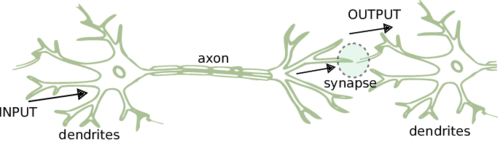
\includegraphics[width=\linewidth]{ANN/images/neural-network.png}
    \caption[Two neurons exchanging information]{
        Information is passed from one neuron to another.
        The message enters the dendrites, passes through the axon, and propagates through the synaptic terminal to another neuron.
        Adapted from \fullcite{Gerstner2002} (Ref.~\cite{Gerstner2002}).
    }
    \label{fig:synapse}
\end{figure}

Inspired by this biological process, artificial neural networks have been developed.
Later, \textcite{Fukushima1980} mimicked this neural network for two dimensional information, using convolution operations.
The approach of \citeauthor{Fukushima1980} was inefficient.
It could not learn to identify reoccurring features.
To enable learning, \textcite{Rumelhart1986} developed backpropagation: an algorithm to learn importances at feature level.
\textcite{LeCun1990} was one of the first to use backpropagation in a visual setting.
They combined convolutions and backpropagation into a convolutional neural network to recognize handwritten digits.

%%%%%%%%%%%%%%%%%%%%%%%%%%%%%%%%%%%%%%%%%%%%%%%%%%%%%%
% BUILDING BLOCKS
%%%%%%%%%%%%%%%%%%%%%%%%%%%%%%%%%%%%%%%%%%%%%%%%%%%%%%

\chapter[CNN building blocks]{The building blocks of convolutional neural networks}

\section{Artificial neural network}
Neural network

\section{Convolutional layers}
To distinguish a neural network from a convolutional neural network (CNN), at least one layer must be a convolution.
A convolution is an operation where a kernel with width $w$ and height $h$ is moved along an input to generate an output.
The output, or output feature map, in two dimensions, is
\begin{equation}
    \mathbf{o}_{i,j} = \mathbf{b}_{i,j} + \sum_{c=0}^{C-1}(\mathbf{x_c} \circledast \mathbf{u}_c)_{i,j}
    = \mathbf{b}_{i,j} + \sum_{c=0}^{C-1}\sum_{n=0}^{w-1}\sum_{m=0}^{h-1}\mathbf{x}_{c,n+i,m+j}\mathbf{u}_{c,n,m},
\end{equation}
where $\mathbf{x}$ is the input possibly containing $C$ multiple channels.
The bias $\mathbf{b}$ and weights $\mathbf{u}$ are learnable parameters.

Convolutions can be modified in a few ways that are important for deep learning.
The first modification is padding, and specifies the size of an added frame around the input.
The frame can have any value, but generally, it is filled with zeros.
A second modification is stride, which specifies the step size with which the kernel moves across the input.

A two-dimensional numerical convolution operation with padding and strides is visualized in \cref{fig:numerical_padding_strides}.
The kernel with size $k=3$ moves across the input of size $i=5$ with stride $s = 2$ in both directions.

Convolutions have the useful property that they are equivariant to translations.
A function $f$ is equivariant to function $g$ if
\begin{equation}
    f \circ g = g \circ f.
\end{equation}
The equivariance of convolutions and translations implies that learned weights and biases belonging to a convolution can be reused for identifying similar features anywhere in inputs.
Moreover, any operator that is not equivariant with convolutions may be used as a way to augment data, as the kernel perceives it is being different.
Examples of such operators are scaling, rotating, and flipping.\marginnote{Move this to its own theory section about data augmentation?}

\begin{figure*}%[p]
    \centering
    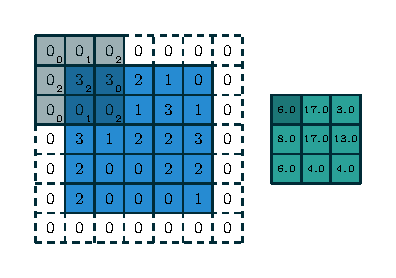
\includegraphics[width=0.32\linewidth]{ANN/images/numerical_padding_strides_00.pdf}
    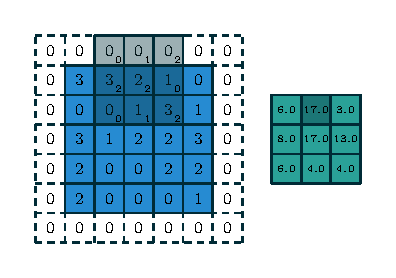
\includegraphics[width=0.32\linewidth]{ANN/images/numerical_padding_strides_01.pdf}
    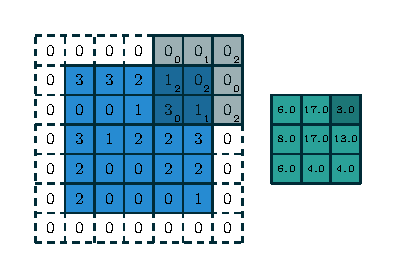
\includegraphics[width=0.32\linewidth]{ANN/images/numerical_padding_strides_02.pdf}
    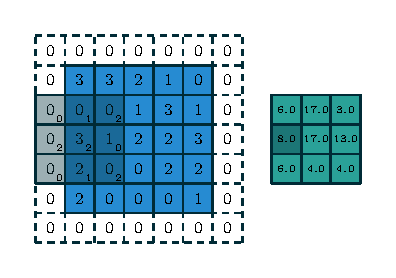
\includegraphics[width=0.32\linewidth]{ANN/images/numerical_padding_strides_03.pdf}
    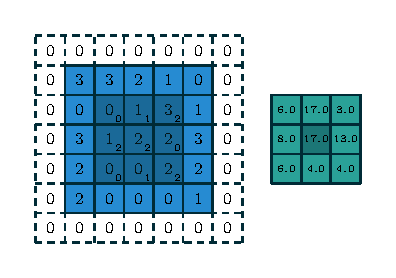
\includegraphics[width=0.32\linewidth]{ANN/images/numerical_padding_strides_04.pdf}
    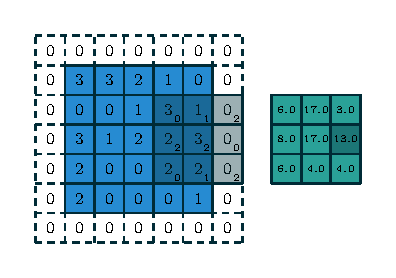
\includegraphics[width=0.32\linewidth]{ANN/images/numerical_padding_strides_05.pdf}
    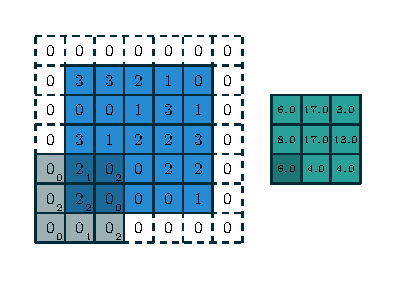
\includegraphics[width=0.32\linewidth]{ANN/images/numerical_padding_strides_06.pdf}
    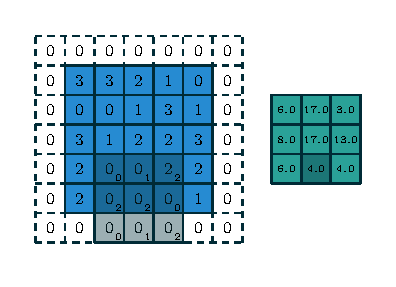
\includegraphics[width=0.32\linewidth]{ANN/images/numerical_padding_strides_07.pdf}
    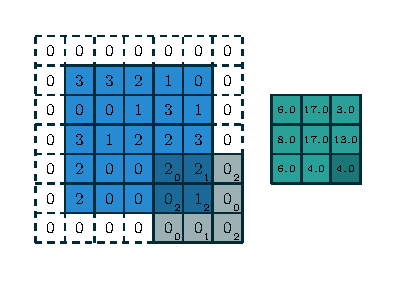
\includegraphics[width=0.32\linewidth]{ANN/images/numerical_padding_strides_08.pdf}
    \caption{Computing the output values
        of a discrete convolution for two dimension, $i_1 = i_2 = 5$, $k_1 = k_2 = 3$,
        $s_1 = s_2 = 2$, and $p_1 = p_2 = 1$.
        Reproduced from \fullcite{Dumoulin2016} (Ref.~\cite{Dumoulin2016}).
    }
    \label{fig:numerical_padding_strides}
\end{figure*}

% \begin{figure*}[p]
%     \centering
%     \includegraphics[width=0.24\textwidth]{ANN/images/arbitrary_padding_no_strides_00.pdf}
%     \includegraphics[width=0.24\textwidth]{ANN/images/arbitrary_padding_no_strides_01.pdf}
%     \includegraphics[width=0.24\textwidth]{ANN/images/arbitrary_padding_no_strides_02.pdf}
%     \includegraphics[width=0.24\textwidth]{ANN/images/arbitrary_padding_no_strides_03.pdf}
%     \caption[Convolution]{
%         Convolving a $4 \times 4$ kernel over a $5 \times 5$ input
%         padded with a $2 \times 2$ border of zeros using unit strides (i.e.,
%         $i = 5$, $k = 4$, $s = 1$ and $p = 2$).
%         Reproduced from \fullcite{Dumoulin2016} (Ref.~\cite{Dumoulin2016}).
%     }
%     \label{fig:arbitrary_padding_no_strides}
% \end{figure*}

\section{Pooling}\label{sec:pooling}
Pooling is a form of nonlinear downsampling.
To achieve this, typically, a convolution kernel is moved over the input with a stride as big as the kernel itself.
This ensures that the downsampling considers measures of input sub-regions.

Pooling is equivariant to any permutation under the kernel.
This results in invariance to local translations.
In deep learning, pooling is therefore used to quantify the presence of a pattern, as opposed to finding its position.

\subsection{Max pooling}\label{subsec:maxpool}
The most common form of pooling is max pooling (ref).
The kernel finds the maximum value in sub-regions and maps these maximum values per sub-region to a new image.
The output
\begin{equation}
    \mathbf{o}_{c, i, j} = \max_{n < h, m < w}\mathbf{x}_{c, si+n, rj+m},
\end{equation}
where $rw$ and $sh$ are the width and height of the input.

\subsection{Average pooling}\label{subsec:avgpool}
Another popular form of pooling is the average pooling, which finds the mean value in sub-regions.
The output
\begin{equation}
    \mathbf{o}_{c, i, j} = \frac{1}{wh}\sum_{n=0}^{w-1}\sum_{m=0}^{h-1}\mathbf{x}_{c,si+n,rj+m}.
\end{equation}

\section{Activation functions}\label{sec:activations}

\begin{enumerate}
    \item heaviside
    \item logistic curves
    \item vanishing gradient problem -> relu
\end{enumerate}

\subsection{Vanishing gradient problem}
Over the years, neural networks have become deeper, \ie more layers are being added.

Sigmoids (and other saturating curves like hyperbolical tangent) have.

\subsection{Rectified linear unit}\label{subsec:relu}
To overcome the vanishing gradient problem, non-saturating activation functions can be used.
One such function is the rectified linear unit (ReLU).
It is defined as
\begin{equation}
    f(x) = x^+ = \max(0, x),
\end{equation}
such that only the positive arguments keep their value.


% --------------------------------------------------
% Loss functions
% --------------------------------------------------

\section{Loss functions}
Backpropagation needs a loss to learn in which direction to update weights.
There is a variety of loss functions available (ref review).

\subsection{Mean absolute error}
One of the most straightforward techniques of calculating the loss is the mean absolute error (MAE).
It measures the average difference between every prediction and target, like
\begin{equation}
    \mathrm{MAE} = \frac{1}{n} \sum_{i=1}^{n} |y_i - y'_i|,
\end{equation}
where $n$ is the number of targets per sample, $y$ the prediction and $y'$ the target.

The MAE loss is forgiving, i.\ e.\ outliers are weighted as much as predictions close to the target.
In training a neural network, focusing on outliers is assumed to be beneficial, as those are the cases that the model has difficulty with (ref).

\subsection{Mean square error}
To overcome the forgiving nature of the MAE loss, the mean square error (MSE) can be used.
It measures the average squared difference between every prediction and target, like
\begin{equation}
    \mathrm{MSE} = \frac{1}{n} \sum_{i=1}^n (y_i - y'_i)^2.
\end{equation}

\subsection{Focal MSE}
To give even more focus on the hard targets, giving them more importance than easy targets can be done through the focal MSE loss (FL)~\cite{Lu2022}.
To give less importance to the easier targets, FL follows
\begin{equation}
    FL = \left(\frac{2}{1 + e^{-\beta |y - y'|}} - 1 \right)^\gamma (y_i - y'_i)^2,
\end{equation}
where increasing $\gamma$ increases the number of targets regarded as easy and $\beta$ regulates the speed with which the first part of the curve increases (make fig).

%%%%%%%%%%%%%%%%%%%%%%%%%%%%%%%%%%%%%%%%%%%%%%%%%%%%%%
% TRAINING A NEURAL NETWORK
%%%%%%%%%%%%%%%%%%%%%%%%%%%%%%%%%%%%%%%%%%%%%%%%%%%%%%

\chapter{Training a neural network}

% --------------------------------------------------
% Hyperparameter optimization
% --------------------------------------------------

\section{Hyperparameter optimization}\label{sec:hparam}

A machine learning model uses training data to learn parameters to map input to output data best.
However, there are parameters that cannot be learned, but greatly influence the training outcome.
These parameters are hyperparameters.
Examples of hyperparameters are the batch size, learning rate, learning rate scheduler and its parameters, optimizer algorithm, etc.
These parameters span a configuration space $\mathcal{C}$.
Parameters can be categoral (type of optimizer, learning rate scheduler, etc.) or integers (batch size, number of iterations, etc.), or continuous decimals (learning rate, weight decay, etc.).
Ideally, parameters are sampled exhaustively.
This way, the best possible set of parameters can be found.
However, this can be computationally expensive.
Moreover, when using a continuous variable, it is no long possible to exhaustively sample parameters.
To engage this problem, various algorithms have been developed to sample hyperparameters from the high-dimensional distribution.

\subsection{Grid search and random search}
The most straightforward technique of finding the best set of hyperparameters is grid search.
With grid search, parameters are sampled exhaustively using equidistant spacing in each dimension.

A drawback of grid search is that optima can reside outside the hyperparameter set that grid search produces.
Random search \cite{Bergstra2012} aims to find optima in the gaps using random search.
With the same number of trials, random search has a higher probability for trials to find the global optimum.
This is because trials explore the whole distribution as opposed to just a few points in individual dimensions.
\Cref{fig:gridrandsearch} shows the differences between grid search and random search and advocates the use of the latter.

\begin{figure}
    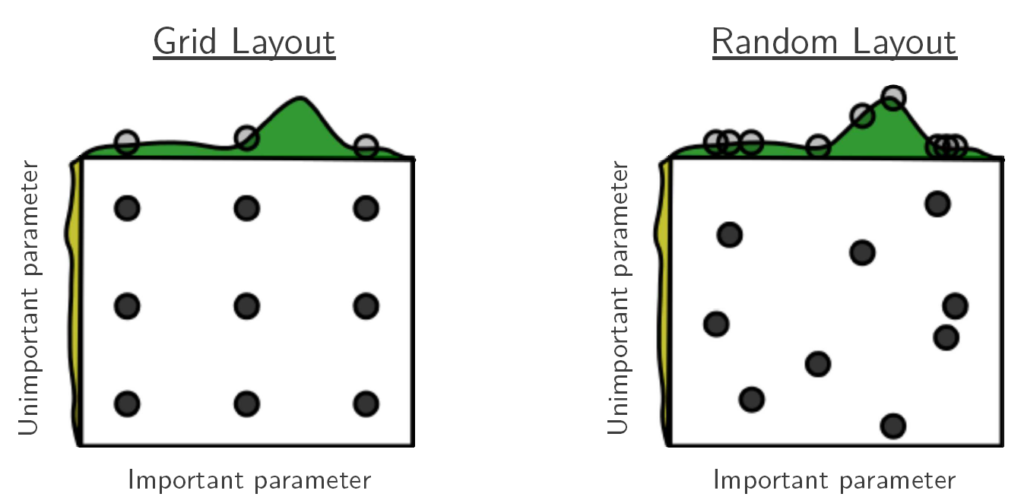
\includegraphics[width=\linewidth]{images/gridrandsearch.png}
    \caption[Grid and random search]{
        Grid and random search of nine trials for optimizing a function $f(x, y) = g(x) + h(y) \approx g(x)$ with low effective dimensionality.
        Above each square $g(x)$ is shown in green, and left of each square $h(y)$ is shown in yellow.
        Reproduced from \fullcite{Bergstra2012} (Ref.~\cite{Bergstra2012}).
    }
    \label{fig:gridrandsearch}
\end{figure}

\subsection{Tree Parzen estimator}
Still, random search requires trials in regions that are unpromising.
This is inefficient.
A tree-structured Parzen estimator (TPE)~\cite{Bergstra2011} approach aims to model the probability of a hyperparameter, given a loss value.
That probability consists of two distributions, describing the good and bad values:
\begin{equation}
    p(c|L) =
    \begin{cases}
        p(c|L > L^*) = p(c|\mathrm{bad}) \\
        p(c|L \leq L^*) = p(c|\mathrm{good}),
    \end{cases}
\end{equation}
where $c$ is drawn from $\mathcal{C}$ and $L$ is the loss.
$L^*$ a loss above which losses are considered bad.
TPE chooses $L^*$ to be a fraction of observed $L$ values, such that $p(\mathrm{good}) = \gamma$.
A promising candidate has low probability under $p(c|\mathrm{bad})$ and high probability under $p(c|\mathrm{good})$.
Therefore, $c$ is promising if
\begin{equation}
    \mathrm{promisingness}(c) \propto p(c|\mathrm{good}) / p(c|\mathrm{bad})
\end{equation}
is high.
Ref.~\cite{Bergstra2011} shows that this ratio is proportional to the expected improvement~\cite{Jones2001}.
The configuration responsible for the maximum of $\mathrm{promisingness}(c)$ is used as the next trial.
Results of that trial are now categorized as good or bad, and the iterative process continues.\marginnote{add multivariate note \cite{Falkner2018}}

\subsection{Successive Halving and Hyperband}
Although $\mathcal{C}$ can be sampled more efficiently with TPE, trials still use the full computational budget, even if it is apparent that the trial is unpromising early on.
Early terminating (or pruning) these underperforming trials speeds up hyperparameter optimization.
Pruning trials can be done using Successive Halving (SH)~\cite{Jamieson2016}.
Given a computational budget $B$, \eg number of epochs, the number of trials $T$, and the halving rate $\gamma$, SH performs $\log_\gamma(T)$ rounds.
The budget is distributed uniformly over the trials.
Every round, $\qty{100}{\percent} \times 1/\gamma$ of the trials are discarded based on their performance.
Surviving trials are allowed twice the budget and are again discarded when they have used up their budget.
This iterative process continues until one trial remains.

When using SH, two variables need to be considered, and possible manually tuned.
The more available budget, pruning decisions are made more confident.
Higher halving rates lead to more and more aggressive pruning with the risk of pruning good candidates early.

There is a trade-off between $T$ and $B$.
Suppose $T$ is large, then each trial gets a small amount of budget, but many configurations are explored.
Conversely, if $T$ is small, then each trial gets much budget, at the cost of exploring the number of configurations.
This $T/B$ trade-off is addressed by Hyperband (HB)~\cite{Li2016} by performing a grid search over feasible values of $T$.
HB invokes SH multiple times.
Every invocation of SH is called a bracket.
In the end, HB returns the best configuration possible just like SH, but diminishing the dependence on manually choosing a good $T$.

\subsection{Parameter importances}
Not every hyperparameter is as important as others.
\textcite{Hutter2014} describe the fANOVA algorithm to quantitatively assess the importance of every hyperparameter.
Knowing the importance of a variable gives more insight into interactions and relative importance between hyperparameters.

\section{Training}\label{Training}
At the start of training, a neural network has its weights and biases initialized.
Most probably, the model is not capable of mapping input to output in a robust manner.
To achieve this, repeatedly using backpropagation to update the model parameters aims to shape the model in the direction of minimizing the loss between target and model output.
The neural network is presented with the input data in batches.
Every batch, the model is updated with the backpropagation algorithm.
One cycle of using all the batches is called an epoch.
A training consists of multiple epochs.

For every $\mathcal{B}$th batch, a loss $\mathcal{L}_\mathcal{B}$ can be defined that is used by backpropagation to penalize the model performance.
Taking the average of all batch losses is the epoch loss,
\begin{equation}
    \mathcal{L}_\mathrm{epoch} = \frac{1}{N_\mathcal{B}}\sum_{i=0}^{N_\mathcal{B}}\mathcal{L}_\mathcal{B},
\end{equation}
Tracking $\mathcal{L}_\mathrm{epoch}$ shows how quickly the model is learning.

To see if the model generalizes, it is standard practice to have a hold-out set, that the model does not learn from, but only uses to calculate the validation loss.
Ideally, this validation loss follows a similar trajectory as the training loss.
If the validation loss diverges upwards from the training loss, the model is overfitting.
It fails to generalize to unseen, but similar data.
To remedy this, there are multiple possible solutions.
Solutions include dropout, batch normalization, or more complex models (\ie deeper or wider networks).

\subsection{Dropout}\label{sec:dropout}
Overfitting can be reduced by applying methods of regularization.
One regularization method is dropout.
It prevents neurons from co-adapting, which would otherwise reduce the chance of the model to perform well on external validation sets \cite{Srivastava2014}.
With dropout, individual neurons are activated with probability $p$, effectively dropping neurons randomly.

\subsection{Batch normalization}\label{sec:bn}
Batch normalization (BN)~\cite{Ioffe2015} is a technique to shift and scale batches akin to standardization.
It can be implemented as a layer in any neural network.
Per minibatch and per dimension, the mean and standard deviation of the input are calculated.
Then, the input is standardized with
\begin{equation}
    \hat{x}_i = \frac{x_i - \mu_\mathcal{B}}{\sqrt{\sigma_\mathcal{B}^2 + \epsilon}},
\end{equation}
where $\mu_\mathcal{B}$ and $\sigma_\mathcal{B}$ are the mean and unbiased standard deviation of the batch, and $\epsilon$ is a small number for numerical stability when the variance is small.
The standardized input is then mapped through
\begin{equation}
    y_i = \gamma \hat{x}_i + \beta,
\end{equation}
where $\gamma$ and $\beta$ are learnable parameters learned in a sub-network.

BN has been shown to have a regularizing effect (ref), although combining it with dropout is disputed.
More often than not, using both BN and dropout leads to worse results on the test set.

\subsection{Model ensembling}\label{subsec:model_ensembling}
A benefit of having a cyclic learning rate is generating multiple models across cycles.
The effectiveness of ensembling models from multiple cycles, Snapshot Ensembling, is first described by \textcite{Huang2017}.
During model training, a model can be checkpointed at the best performing epoch for every cycle, see \.
The checkpointed models can be ensembled by choosing the last $m$\marginnote{how many models chosen and how many models checkpointed then?!} out of $n$ models and averaging the output, as
\begin{equation}
    \mathrm{output} = \frac{1}{M} \sum_{i=0}^{m-1} \mathrm{model}_{n-i}(\mathrm{input}).
\end{equation}
\begin{figure}
    \centering
    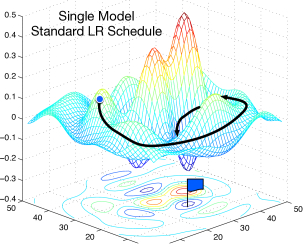
\includegraphics[width=0.48\linewidth]{ANN/images/ensembling_huang_left.png}
    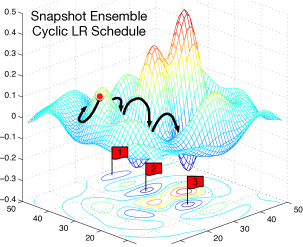
\includegraphics[width=0.48\linewidth]{ANN/images/ensembling_huang_right.png}
    \caption[Snapshot ensembling]{
        Left: Illustration of model optimization The model converges to a local minimum.
        Right: Illustration of Snapshot Ensembling.
        The learning rate is cyclic and annealing, allowing to converge to and escaping from local minima.
        Snapshots are taken at every minimum which can be used for ensembling for inference.
        Reproduced from \fullcite{Huang2017} (Ref.~\cite{Huang2017}).
    }
\end{figure}


% --------------------------------------------------
% Image quality
% --------------------------------------------------

\section{Image quality}\label{subsec:imq}
A convolutional neurel network receives a stream of input images with varying quality.
For example, microscopy images from deep inside tissue are presumably noisier and/or less bright than images taken near the surface.
Neural networks have trouble learning from bad images, as they lack structures that trigger neurons to output predictions close to targets.
Excluding noisy images might increase performance \cite{Blokker2022}.
\textcite{Koho2016} suggest some measures to quantify image quality.
Here, the entropy and kurtosis are discussed.

\subsection{Shannon entropy}
The quality of an image may be described by the amount of information that is contained within it.
The information can be quantified by how surprising it is to contain specific content.
For instance, knowledge that a rare event will occur has high informational value, while knowledge that a probable event will happen has low informational value.
Given a random variable $X$, the information, or entropy, is defined as
\begin{equation}\label{eq:entropy}
    H = \mathbb{E}[-\log p(X)] = -\sum p(x) \log p(x),
\end{equation}
where $\mathbb{E}[\ldots]$ is the expectation operator, and $p(x)$ is the probability of $x$ occurring.
The logarithm satisfies the boundary condition that an event is not surprising if its probability of occurring is one.

For images, \cref{eq:entropy} can be rewritten as
\begin{equation}
    H_I = -\sum_{i}^n P_i \log_2 P_i,
\end{equation}
where $P_i$ is the normalized image histogram at bin index $i$ \cite{Koho2016}.
The base of the logarithm is chosen to be two, such that the entropy is in units of bits.

For images having many different intensities, the entropy is high, because of the knowledge that pixel intensities having lower probability.
The intuition for images with high entropy tending to carry more information is the same as taking images with longer exposure times:
the number of pixels with a certain intensity will increase.
This may be most apparent in dark regions, which would benefit from more illumination.

\subsection{Kurtosis}
Another measure for image quality is kurtosis of the power spectrum.
Kurtosis measures the outliers of a distribution and is given by
\begin{equation}
    \kappa = \frac{\mu_4}{\sigma^4},
\end{equation}
where $\sigma$ is the standard deviation and $\mu_4$ is the fourth moment about the mean.
The $n$th moment about the mean is defined as
\begin{equation}
    \mu_n = \mathbb{E}[(X-\mathbb{E}[X])^n] = \int_{-\infty}^\infty (x-\mu)^n p(x)\,\mathrm{d}x.
\end{equation}
Distributions having a kurtosis of zero are mesokurtic, meaning they resemble a normal distribution.
Posivite kurtosis means that the distribution is leptokurtic.
A leptokurtic distribution has tails with more weight compared to the normal distribution, such as the Poisson or Laplace distribution.
Negative kurtosis means that the distribution is platykurtic.
Platykurtic distributions have thinner tails, such as the Bernoulli distribution.

Kurtosis can be calculated on the upper part of the power spectrum of an image \cite{Koho2016,Blokker2022}.
If the upper part of the power spectrum is very leptokurtic compared to other images in the dataset, it may indicate that the image is an outlier and is significantly different from the mean.

\section{Explainable AI}
A significant number of users of a trained AI generally view the model as a black box that simply maps input to output.
How this box is constructed and why it results in a particular outcome is often overlooked.\marginnote{ref!}
Meanwhile, techniques to give insight into the black box (explainable AI, XAI) have been developed.
These techniques fall in roughly two categories: gradient and perturbation based methods.
Gradient based methods rely on gradients calculated during the backward pass and use these to find which parts of the input contribute to the output most.
Perturbation methods perturb the input to see how the output changes.
Large output changes yield large attributions.

Explainability is particularly important in clinical settings where merely relying on AI output is sometimes unethical.
AI solutions exist that predict patient outcome after new treatment given current health status [refs] or segment tumour regions in medical imaging after which the predicted region will be excised or treated with radiotherapy.
XAI gives users and patients more confidence in the prediction so that specialists can proceed with treatment.

\subsection{Occlusion}\label{subsec:occlusion}
Occlusion \cite{Zeiler2013} is an XAI pertubation technique.
The method replaces patches of the input with a baseline value.
\eg for images, patches can consist of any shape and the baseline value can be 0, practically making a patch black and removing all information at the patch's location and the connections with neighbouring pixels.
In the original paper, occlusion is used to systematically cover parts of foreground objects, to gain confidence in the AI using foreground objects to predict the output.
If the AI still recognizes an object from an image where the object has been cut out, the AI may use background for its prediction.

A generalized occlusion algorithm includes a moving patch.
The patch, mostly a rectangle of a given size and value, is placed on the image.
The AI computes an output, given the masked input.
The masked output is subtracted from the original output.
This difference divided by the patch size is assigned to the patch.
A new patch is placed and the iterative process continues until the patches have been placed on all possible input locations.


% \pagelayout{wide} % No margins
% % \addpart[Skinstression]{Strain-stress regression on \\ second harmonic generation images \\ using {\normalfont\textsc{Skinstression}}}
% \addpart[Skinstression]{Developing and validating a strain-stress regression model on second harmonic generation images from old adult skin tissue}
% \pagelayout{margin} % Restore margins

\pagelayout{wide}
\chapter[Skinstression]{Developing and validating a strain-stress regression model on second harmonic generation images from old adult skin tissue}
\pagelayout{margin} % Restore margins

\section{Introduction}

Human skin tissue is built by a series of layers, one of which is the dermis layer.
The dermis contains a network of collagen fibrils, dictating the stretch of skin tissue.
Measuring the strain-stress response of skin tissue gives insight into the skin's strength and elasticity that protects the body from external forces.
A recent study (Mengyao) aims to show the connection between collagen density and stretch.
To measure the strain-stress response of skin tissue, mechanical measurements have to be performed.

Second harmonic generation (SHG) imaging allows imaging collagen and two-photon excitation microscopy (2PEF) elastin.
Setups have been built to collect SHG and 2PEF signals simultaneously, allowing for rich skin tissue imaging.
Collagen fibers are clearly visible.
% Previous studies have shown that collagen and not elastin dictates the stretching ability of skin tissue.
SHG images of the collagen networks in conjunction with the strain-stress curves suggest that the images already contain stretch information.
Retrieving complex features from labelled images can be done using supervised deep learning.
Supervised deep learning is considered a black-box technique that aims to learn a mapping from input to output.
With the SHG images and corresponding stress-strain measurements at hand, Skinstression (from skin stretch regression) is developed with the ultimate goal to replace mechanical measurements on skin tissue to quantify skin stretch.
Possibly, the model can be used to non-invasively investigate physical parameters to aid plastic surgery.
For example, the prior flexibility of skin tissue determines the amount of manual continuous or cyclic stretching needed to close a gap after excision~\cite{Verhaegen2012}.

Efforts to develop such a model have already been made by Soylu~\cite{Soylu2022}.
However, those methods do not consider complete separation of training and test sets in both inference and label creation, possibly leading to biased results.
Moreover, only one slice of larger image stacks have been used.
The original model does not incorporate physical properties of the strain-stress curves but relies on principal component analysis.

Frequently, machine learning models and neural networks in particular lack the ability to explain how the model comes to its conclusions.
Meanwhile, explainable artificial intelligence (XAI) techniques exist to shed light on the inner workings of algorithms, but are used sparingly.
In the context of skin tissue, XAI could give insight into where the strength and elasticity comes from.
A human expert might recognize straight collagen fibrils as a stiff network~\cite{Holzapfel2001}, but it is interesting to see if an AI explains stiffness in the same manner.

The objective of this study is to extend Soylu's model.
To this end, an application, Skinstression, will be developed and validated with separate training and validation data.
A new, physics informed neural network will be implemented for explainability.
The data will not only consist of single slices from depth scans, but of subsets considering multiple slices per depth scan.
Moreover, XAI procedures will be adopted to better explain the black box output.

The purpose of the product is to accompany or possibly replace mechanical strain-stress measurements on skin tissue.
Explainability techniques might shed light on how top level collagen structures provide strength and elasticity to skin.
Unintentionally, the project may be used more generally to train other convolutional neural networks for regression.

\section{Theory}

% In addition to the theory described in \cref{ch:theory}, this section describes theory only applicable to the Skinstression project.
% \subsection{Collagen}
% TODO. How does it look like in SHG imaging?

% --------------------------------------------------
% SEARCHING FOR A SIMPLE SKIN STRAIN-STRESS MODEL
% --------------------------------------------------

\subsection{Searching for a simple skin strain-stress model}\label{subsec:skin_predictors}

Supervised learning requires targets for the model to train on.
Ideally, individual targets allow for physical interpretation and can together describe all the available data.

\subsubsection{Empirical strain-stress regions}
Although skin tissue has a complex nature, measurements to quantify skin stretch show similar features.
Measurements show four domains: the toe, heel, leg and break domain (\cref{fig:stress-strain-curve-skin-tissue}A).
The toe region is at the very start of the curve.
This region is relatively flat as the fiber network consists of mostly straight fibers.
Therefore, the fibers cannot exert force as a reaction to external stretching force.
However, in the heel region where skin tissue is stretched more, fibers can exert more force.
When enough force is exerted on the tissue, fibers stretch maximally and fibers react with maximum force in the leg region.
This region is observed to be roughly linear.
Overstretching the tissue then breaks the fiber network, decreasing the possibility to exert force.

\begin{figure}
    \centering
    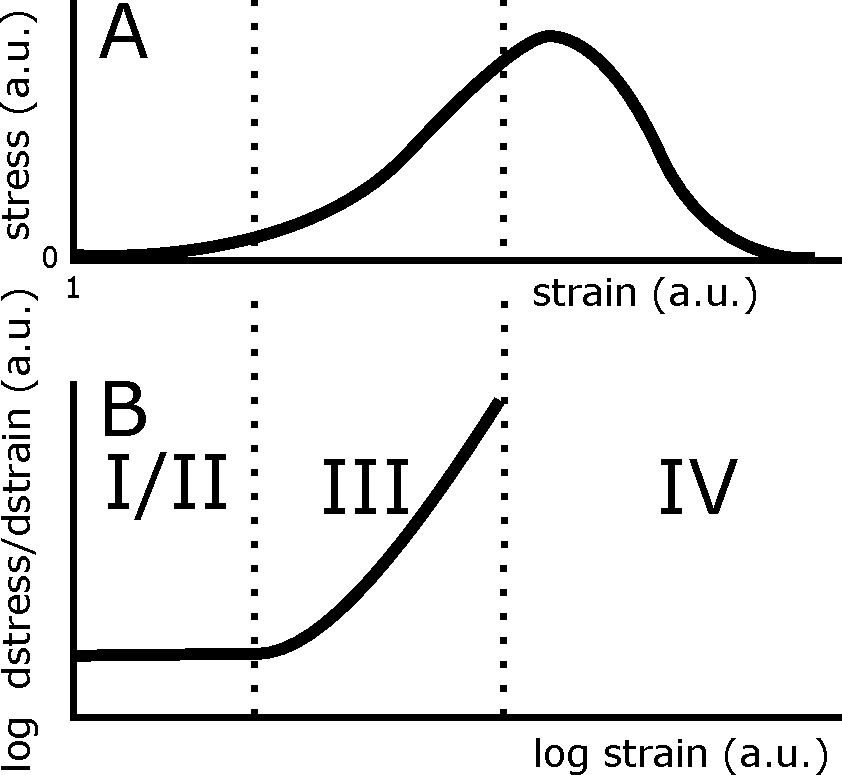
\includegraphics[width=\linewidth]{skinstression/images/stress-strain-curve.pdf}
    \caption[Stress-strain curve of human skin tissue]{
        Stress-strain curve of human skin tissue.
        The curve is divided in three regions.
        I: the toe region.
        The fiber structure here consists of mostly straight fibers.
        II: the heel region.
        Fibers begin to stretch.
        III: the leg region.
        Fibers stretch maximally and react with maximum force.
        IV: break region.
        Fibers break and give up ability of applying force.
    }
    \label{fig:stress-strain-curve-skin-tissue}
\end{figure}

\subsubsection{Exponential}\label{subsubsec:exp}
Strain-stress curves can also be visualized by showing the log derivative of stress with respect to strain against the log of strain as in \cref{fig:stress-strain-curve-skin-tissue}B.
Typically, this figure has three regions.
The first region indicates a linear relationship between small forces and small strain.
Then, the derivative increases until it reaches a purely exponential part~\sidecite{Holzapfel2001}.
If skin stretching follows this kind of behavior, a simple mathematical model can be derived.
Inspecting the figure, the linear part shows the ordinary differential equation
\begin{equation}
    \frac{\mathrm{d}\sigma}{\mathrm{d}\gamma} \propto \sigma,
\end{equation}
where $\gamma = \chi - 1$.
Solving for $\sigma$, we get
\begin{equation}
    \sigma \propto e^{\lambda\gamma},
\end{equation}
where $\lambda$ is some factor dictating the speed with which the exponential increases.
At no extension, $\gamma=0$, it can be assumed that there is no stress.
Therefore,
\begin{equation}
    \sigma \propto e^{\lambda\gamma} - 1.
\end{equation}
At small extensions, $\lambda\gamma \ll 1$, $e^{\lambda\gamma} \approx (1 + \lambda\gamma + \ldots)$ using a Taylor expansion.
So
\begin{equation}
    \sigma_{\lambda\gamma\ll 1} \propto 1 + \lambda\gamma + \ldots - 1 \approx G_0 \gamma,
\end{equation}
where $G_0$ is some linear coefficient at small extensions.
In this work, $\gamma = \chi - 1$, where $\chi$ is the stretch.
The full expression then becomes
\begin{equation}\label{eq:exp}
    \sigma = \frac{G_0}{\lambda}\left(e^{\lambda(\chi - 1)}-1\right).
\end{equation}

This model assumes that data follows the previously described curve where there is a small rise at small extensions and an indefinitely exponentially increasing stress for larger extensions.

The exponential model is fit to some stress-strain curves using OriginPro~\sidecite{OriginPro}.

\subsubsection{Principal component analysis}
In an earlier study \sidecite{Soylu2022}, principal component analysis (PCA) is used to reduce the dimensionality of the strain-stress data.
In summary, after PCA, every measurement $Y$ can be approximated by
\begin{equation}\label{eq:pca}
    Y \approx Y_\mathrm{PCA} = \mathbf{A} \mathbf{V} + \bar{Y},
\end{equation}
where $\mathbf{A}$ and $\mathbf{V}$ are matrices containing respectively the eigenvalues and eigenvectors of the measurement data.
$\bar{Y}$ is the measurement mean.
Choosing the first $p$ principal components allows for dimensionality reduction.

Using PCA to create eigenvalues to weight the eigenvectors has some caveats.
First, the training and test sets must be treated separately.
The test set has to be projected on the space spanned by the first $p$ eigenvectors of the training set.
This may induce problems as the test set could contain information that does not come close to
Second, PCA depends on interpolation, \ie every strain-stress curve must be formed by either a set of strain or stress values.
This reduces the domain of the data.

\paragraph{Logistic curve}
The empirical observations where the force response of skin tissue changes states, suggests a logistic curve, which can be written as
\begin{equation}\label{eq:logistic_curve}
    \sigma = \frac{\sigma_\mathrm{max}}{1+e^{-E_\mathrm{max} (\gamma - \gamma_c)}},
\end{equation}
where $\sigma$ and $\gamma$ are the stress and engineering strain, $\sigma_\mathrm{max}$ is the maximum stress, $E_\mathrm{max}$ is the maximum Young's modulus and $\gamma_c$ the strain offset.
This equation assumes that there is a maximum force that the tissue can exert, in contrary to the theoretical approach in \cref{subsubsec:exp}.

Using the logistic curve as an alternative to PCA has two major advantages.
Every curve can be treated separately and measurements can contain data across arbitrary domains and with arbitrary intervals as no interpolation is necessary.

% --------------------------------------------------
% Label density smoothing
% --------------------------------------------------

\subsection{Label density smoothing}
The targets calculated with logistic curve fitting result in a non-uniform distribution.
Data imbalance reduces the ability of a neural network to learn outliers.
This may have significant impact on the test results.
To deal with imbalanced data, various techniques have been developed.
One of those techniques is label density smoothing (LDS)~\sidecite{yang2021delving}.
It is specifically designed for deep neural networks to learn from imbalanced continuous targets.

\newcommand{\edtl}{$\tilde{p}(y')$ }
LDS computes the effective label density distribution,
\begin{equation}
    \tilde{p}(y') = \int_Y k(y, y')p(y)dy,
\end{equation}
where $k(y,y')$ is a symmetric kernel, $p(y)$ the number of label $y$ present in the training data and \edtl the effective density of target label $y'$.
Reweighting the loss function with the inverse (square root) of \edtl addresses target imbalance.

\subsection{Goodness of fit}\label{subsec:coef_det}

% \subsubsection{Coefficient of determination}\label{subsec:coef_det}
One possible way to quantify how good a fit is, is to calculate the coefficient of determination.
The coefficient of determination of a dataset $y$ and its prediction $f$, is calculated with
\begin{equation}
    R^2 = 1 - \frac{SS_\mathrm{tot}}{SS_\mathrm{res}},
\end{equation}
where
\begin{equation}
    SS_\mathrm{tot} = \sum_i (y_i - \bar{y})^2,
\end{equation}
with $\bar{y}$ the mean of $y$, and
\begin{equation}
    SS_\mathrm{res} = \sum_i (y_i - f_i)^2.
\end{equation}

If $R^2 = 1$, the prediction perfectly fits the data.
There are some caveats to using $R^2$ to determine the goodness of fit.
Most notably, $R^2$ does not indicate whether the model is the correct model or whether there are enough data points to draw a conclusion.

\section{Methods}
\begin{enumerate}
    \item TODO: SQUASH SECTION BELOW INTO FEWER SECTIONS AND MAKE IT FLOW
    \item TODO: DETAIL
\end{enumerate}

\subsection{Sources of data}

Data is obtained in previous studies by A.\ Soylu, M.\ Zhou, and Ludo X\marginnote{What is Ludo's name? And ref to paper?} at the Medical Imaging center of the VUmc, Amsterdam.
\marginnote{Agreement?}
Human thigh and abdomen skin tissue were excised.
Pieces of these tissues were imaged with multiphoton microscopy and their stress-strain response curves were measured mechanically.
Data is acquired in batches from April 2021 until July 2022.
Development and testing data come from the same source.

Cadavers were eligible for thigh skin excision and abdomen skin is cut during plastic surgery.\marginnote{is this true?}
It is unknown if individuals received treatment relevant for this study.


\subsection{Data preparation}\label{sec:skin_data_prep}

\subsubsection{Preprocessing}

Depth stack images with a size of $\qty{1000}{px}\times\qty{1000}{px}$of all skin tissues were kindly provided by M.\ Zhou.
All stacks were separated into slices.

Images consist of three channels: third and second harmonic generation, and autofluorescence.
The SHG channel is chosen as it is assumed to only contain collagen information.

The SHG images are enhanced with contrast limited adaptive histogram equalization (CLAHE) \cite{Zuiderveld1994ContrastLA} using scikit-image \cite{scikit-image} to equalize importance of dark and bright regions.

The enhanced images are then transformed with a Yeo-Johnson transform using Scipy \cite{2020SciPy-NMeth} such that the histogram of all images is as normal as possible.

The transformed images are standardized by subtracting the total mean and total standard deviation of the complete transformed image set, like
\begin{equation}
    X_\mathrm{out} = \frac{X_\mathrm{in} - \mu}{\sigma},
\end{equation}
where
\begin{equation}
    \mu = \frac{1}{N} \sum_i \sum_j \sum_k X_{i,j,k},
\end{equation}
and
\begin{equation}
    % \sigma = \sqrt{\frac{1}{N} \sum_{i,j,k} X_{i,j,k}^2 - \left(\frac{1}{N} \sum_{i,j,k} X_{i,j,k}\right)^2},
    \sigma = \sqrt{\frac{1}{N} \sum_i \sum_j \sum_k \left(X_{i,j,k} - \mu\right)^2},
\end{equation}
with $N$ the total number of pixels, $k$ an individual image and $i,j$ the pixel in the horizontal and vertical dimension, respectively.

The images are downsampled to $\qty{258}{px}\times \qty{258}{px}$ to fit into the neural network.

\subsubsection{Image selection}
SHG microscopy images from skin tissue suffer from optical phenomena.
The most evident problem is that imaging deeper into the tissue, photons are detected with less spatial accuracy thanks to scattering.
The deeper photons travel into tissue, the more possible paths photons can take to return to the detector.
Moreover, the chance of photons getting absorbed by the tissue increases with penetration depth.
Therefore, less photons get reflected from deeper tissue.

To counter these optical effects, inspired by \textcite{Koho2016} and \textcite{Blokker2022}, measures to quantify image quality can be obtained.
With this, images can be sorted to this measure and the top $k$ images with best quality can be used to train the network, thus excluding noise.

Candidates for this measure are Shannon entropy, kurtosis, and skew for reasons explained in \ref{subsec:imq}
These quality measures are calculated per image using PyImageQualityRanking \cite{Koho2016}, such that the quality measure can be validated by observing manually.

\subsubsection{Image denoising}
Another optical disadvantage of multiphoton microscopy is the occurrence of noise.\marginnote{Look up sources of noise.}

Unfortunately, obtaining clearer images is hard.
Given the experimental setup as in (ref\marginnote{Actually refer to the paper describing the setup, which is written by whom?!}), one way to reduce noise in the image is to use more photons.
Either by averaging more images or increasing the amount of photons per image.
Increasing the amount of photons penetrating the tissue increase the risk of damaging the tissue.

Another way to deal with noisy images is to process the images.
Promising denoising neural networks have been developed.
The difficulty with this is that clean target data for supervised training is often not available in a biomedical setting.
To counteract this, Noise2Noise (N2N) \cite{Lehtinen2018} was developed.
Noise2Void N2V \cite{Krull2019}, a successor of N2N, does not rely on pairs of noisy images.
Instead it only needs one image and corrupts it to use as target and learns a mapping between the noisy image and the newly created noisy image.
This is useful if only one biomedical image is available.\marginnote{If denoised is used, move parts of this section to a theory section and refer to it here.}

The original N2V model produces a checkerboard pattern.
Noise2Void2 (N2V2) \cite{Hock2022} is an extension to N2V and reduces this artifact.\marginnote{Actually didn't do denoising, but if done, describe how here :)}

\subsubsection{Data augmentation}

To make the model more robust, data augmentation is applied.
Before the downsampling, the preprocessed images are cropped randomly from $\qty{1000}{px}\times \qty{1000}{px}$ to $\qty{700}{px}\times \qty{700}{px}$ preserving the aspect ratio.
The global brightness is adjusted randomly with $\pm \qty{30}{\percent}$.
The images are then randomly mirrored horizontally and vertically with a probability of \qty{50}{\percent}.
All data augmentations were performed with Torchvision \cite{torchvision2016}.

\subsection{Outcome}
The strain-stress response curves of individual skin tissue pieces were the outcome of interest.
The prediction is assessed by comparing it with measured strain-stress curves.\marginnote{Describe this comparison}
The measurement is done mechanically by an experimentalist.
The mechanical measurement itself is blind to clinical information.

\subsection{Predictors}\label{sec:skin_predictors}

% --------------------------------------------------
% SEARCHING FOR A SIMPLE SKIN STRAIN-STRESS MODEL
% --------------------------------------------------

\subsubsection{Searching for a simple skin strain-stress model}

Supervised learning requires targets for the model to train on.
Ideally, individual targets allow for physical interpretation and can together describe all the available data.

\paragraph{Empirical strain-stress regions}
Although skin tissue has a complex nature, measurements to quantify skin stretch show similar features.
Measurements always show three domains: the toe, heel and leg domain (see fig.).
The toe region is at the very start of the curve.
This region is seems relatively flat as the fiber network consists of mostly unstretched fibers.
Therefore, the fibers cannot exert force as a reaction to external stretching force.
However, in the heel region where skin tissue is stretched more, fibers can exert more force.
When enough force is exerted on the tissue, fibers stretch maximally and fibers react with maximum force in the leg region.
This region is observed to be roughly linear.
Overstretching the tissue then breaks the fiber network, decreasing the possibility to exert force.

\paragraph{Exponential}
Strain-stress curves can be also be visualized by showing the log derivative of stress with respect to strain against the log of strain (fig).
Typically, this figure has three regions.
The first region indicates a linear relationship between small forces and small strain.
Then, the derivative increases until it reaches a purely exponential part.
If skin stretching follows this kind of behaviour, a simple mathematical model can be derived.
Inspecting the figure, the linear part shows the ordinary differential equation
\begin{equation}
    \frac{\mathrm{d}\sigma}{\mathrm{d}\gamma} \propto \sigma,
\end{equation}
where $\gamma = \chi - 1$.
Solving for $\sigma$, we get
\begin{equation}
    \sigma \propto e^{\lambda\gamma},
\end{equation}
where $\lambda$ is some factor dictating the speed with which the exponential increases.
At no extension, i.\ e.\ $\gamma=0$, it can be assumed that there is no stress.
Therefore,
\begin{equation}
    \sigma \propto e^{\lambda\gamma} - 1.
\end{equation}
At small extensions, i.\ e.\ $\lambda\gamma \ll 1$, $e^{\lambda\gamma} \approx (1 + \lambda\gamma + \ldots)$ using a Taylor expansion.
So
\begin{equation}
    \sigma_{\lambda\gamma\ll 1} \propto 1 + \lambda\gamma + \ldots - 1 \approx G_0 \gamma,
\end{equation}
where $G_0$ is some linear coefficient at small extensions.
In this work, $\gamma = \chi - 1$, where $\chi$ is the stretch.
The full expression then becomes
\begin{equation}\label{eq:exp}
    \sigma = \frac{G_0}{\lambda}\left(e^{\lambda(\chi - 1)}-1\right).
\end{equation}

This model assumes that data follows the previously described curve where there is a small rise at small extensions and an indefinitely exponentially increasing stress for larger extensions.

The exponential model is fit to some stress-strain curves using OriginPro~\cite{OriginPro}.

\paragraph{Principal component analysis}
In an earlier study \cite{Soylu2022}, principal component analysis (PCA) is used to reduce the dimensionality of the strain-stress data.
In summary, after PCA, every measurement $Y$ can be approximated by
\begin{equation}\label{eq:pca}
    Y \approx Y_\mathrm{PCA} = \mathbf{A} \mathbf{V} + \bar{Y},
\end{equation}
where $\mathbf{A}$ and $\mathbf{V}$ are matrices containing respectively the eigenvalues and -vectors of the the measurement data.
$\bar{Y}$ is the measurement mean.
Choosing the first $p$ principal components allows for dimensionality reduction.

Using PCA to create eigenvalues to weight the eigenvectors has some caveats.
First, the training and test sets must be treated separately.
The test set has to be projected on the space spanned by the first $p$ eigenvectors of the training set.
This may induce problems as the test set could contain information that does not come close to
Second, PCA depends on interpolation, \ie every strain-stress curve must be formed by either a set of strain or stress values.
This reduces the domain of the data.

\paragraph{Logistic curve}
The empirical observations where the force response of skin tissue changes states, suggests a logistic curve, which can be written as
\begin{equation}\label{eq:logistic_curve}
    \sigma = \frac{\sigma_\mathrm{max}}{1+e^{-E_\mathrm{max} (\gamma - \gamma_c)}},
\end{equation}
where $\sigma$ and $\gamma$ are the stress and engineering strain, $\sigma_\mathrm{max}$ is the maximum stress, $E_\mathrm{max}$ is the maximum Young's modulus and $\gamma_c$ the strain offset.
This equation assumes that there is a maximum force that the tissue can exert, in contrary to the theoretical approach above (ref).

Using the logistic curve as an alternative to PCA has two major advantages.
Every curve can be treated separately and measurements can contain data across arbitrary domains and with arbitrary intervals as no interpolation is necessary.

Strain-stress curves for all individuals were kindly provided by M.\ Zhou.
The curves only include datapoints where the skin extension is larger than zero and the force positive.

To every strain-stress curve, eq.~\ref{eq:logistic_curve} is fitted with Scipy \cite{2020SciPy-NMeth}.
The optimal parameters were be used for training the model.

BIAS\marginnote{Include density/thickness analysis of Mengyao and the gender/age analysis of myself}

The AI was trained on a with LDS smoothed target variable distribution.
The targets were weighted with the inverse square root, to limit the impact of LDS.

\subsection{Sample size}
The sample size is arrived at taking into account all previously included subjects (ref ludo, ref mengyao, ref alperen) and excluding abdomen data.
This amounts to a total of 1649 SHG images to train on.
For a detailed summary of the number of samples, see fig. (graph with nodes and edges explaining number of images/curves).

\subsection{Missing data}
Due to the limited amount of participants, individuals with unknown gender or age were included.

\subsection{Statistical analysis methods}

This section shows the methods obtain a trained model from stress-strain curves and images to use it for inference and interrogate it with XAI techniques.
The statistical methods are summarized in \cref{fig:skin_stat_methods}.

\begin{figure*}[p]
    \centering
    % 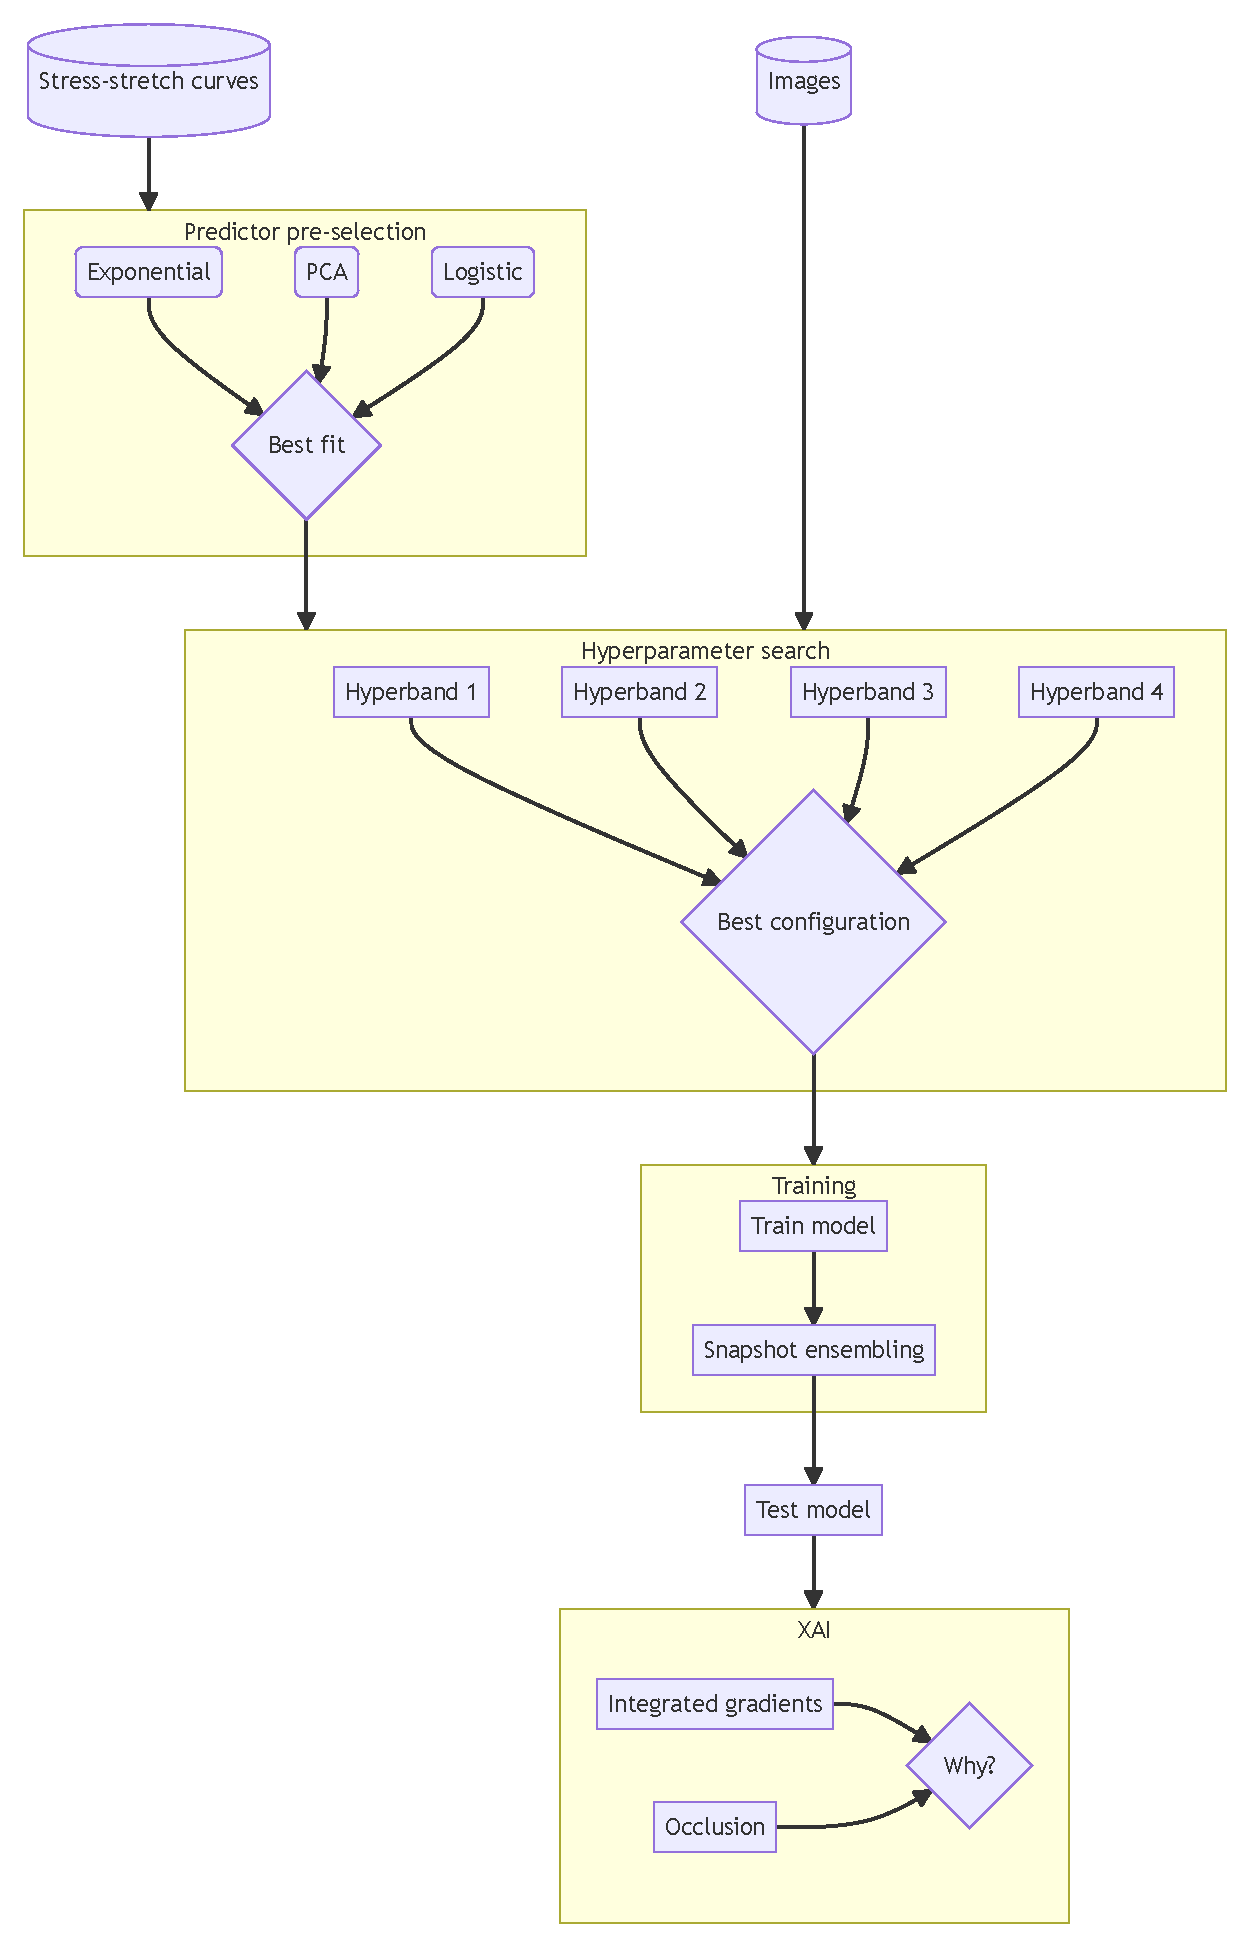
\includegraphics[height=\dimexpr\textheight-55.89pt\relax]{mermaid/skin_analysis.pdf}
    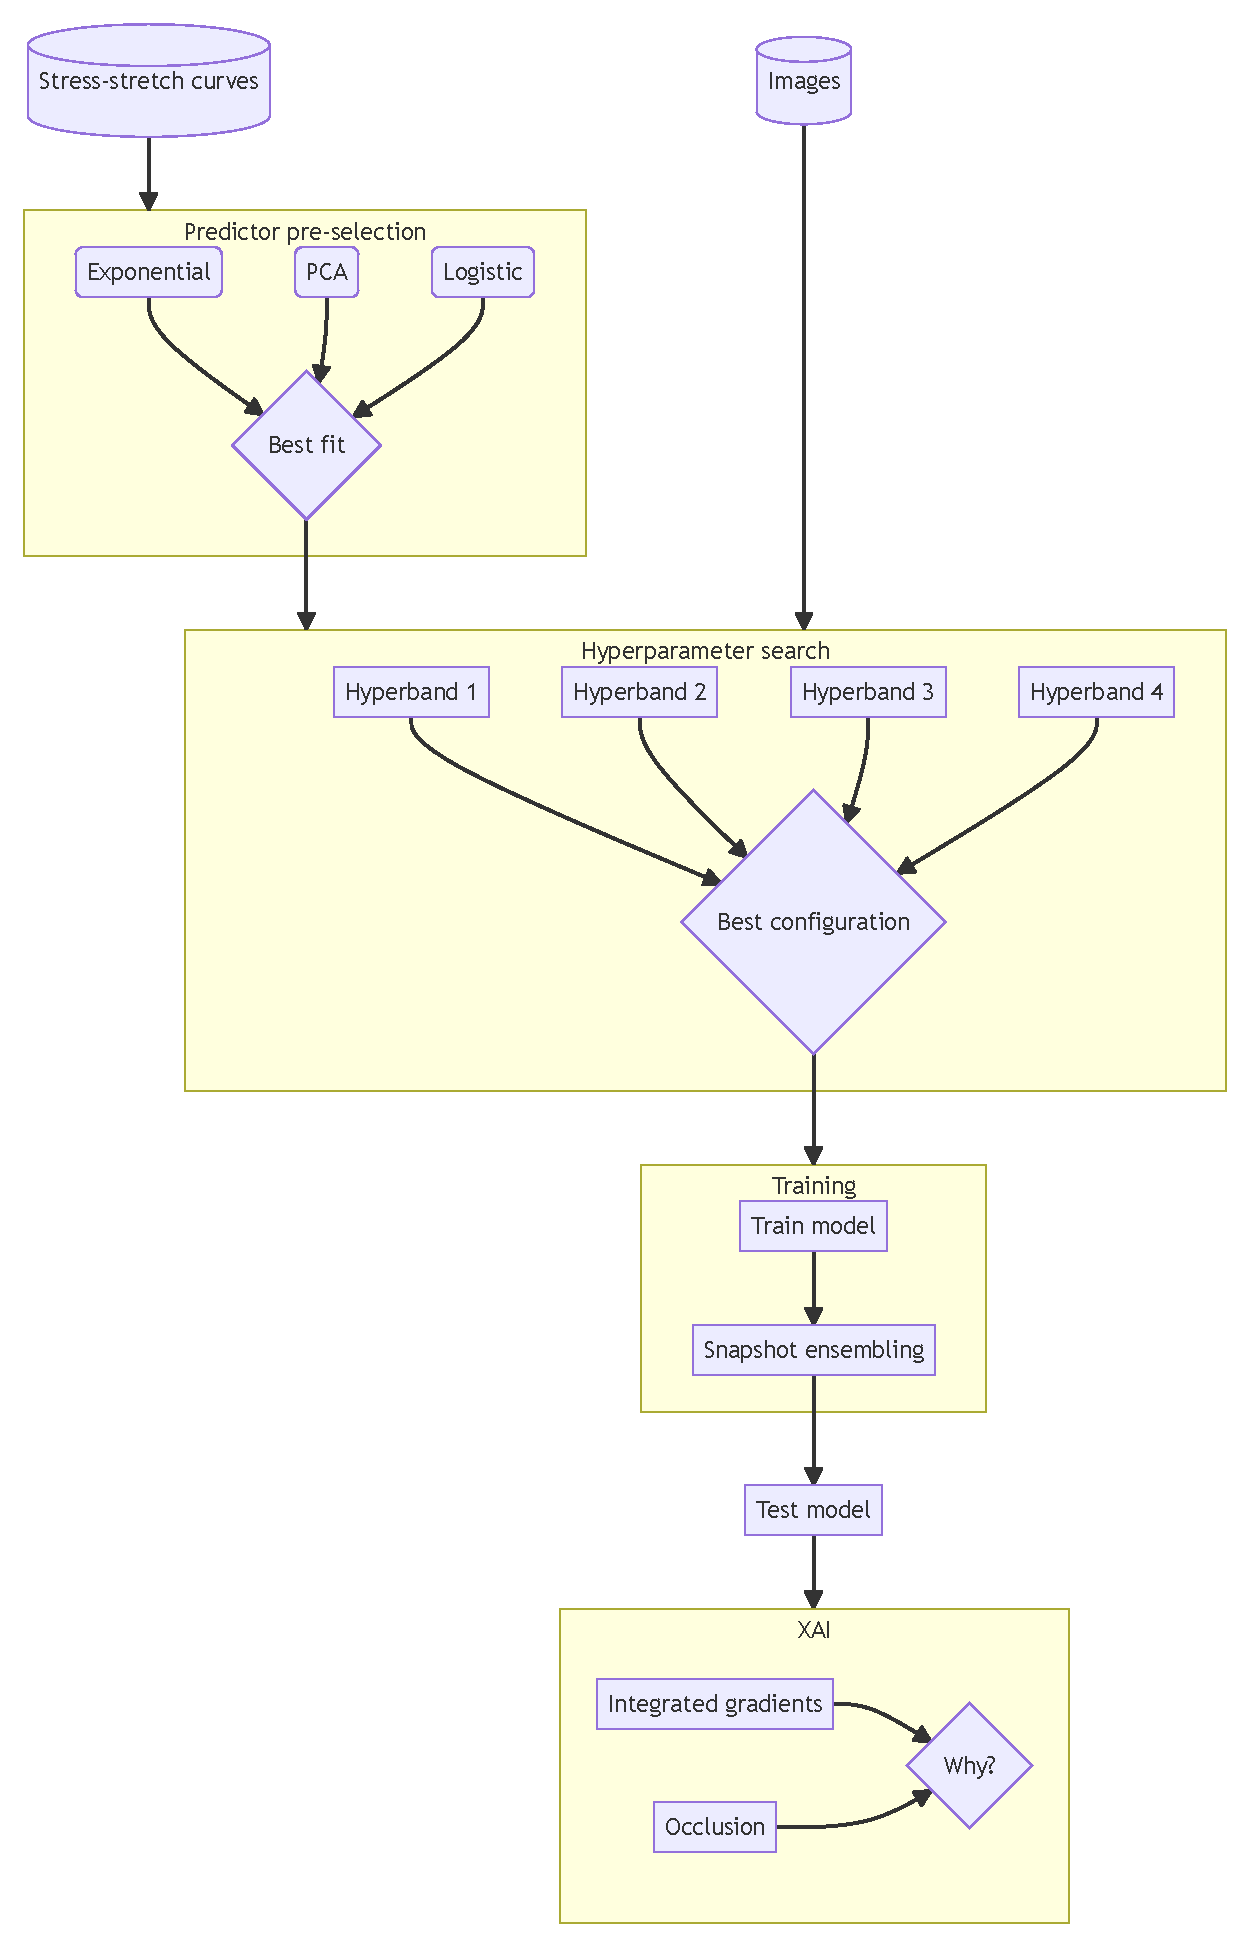
\includegraphics{mermaid/skin_analysis.pdf}
    \caption[Flowchart of statistical analysis methods for \textsc{Skinstression}]{
        Flowchart of statistical analysis methods for \textsc{Skinstression}.
        Exponentials, principal component analysis (PCA) reconstructions, and logistic curves were fit to the stress-strain curves.
        The best-fitted model was used to create training targets.
        The targets and images were used as input for further training.
        The hyperparameter search was performed by four Hyperband studies and the best configuration was used to train four models.
        The best validation loss determines the final model.
        The final model is tested and interrogated using occlusion and an adversarial attack.
    }
    \label{fig:skin_stat_methods}
\end{figure*}

\subsubsection{Predictor pre-selection}
As discussed in \cref{sec:skin_predictors}, there are three predictor candidates.
These candidates are tested against the original strain-stress curves.

\paragraph{Exponential and logistic curve}
The exponential and logistic models are fitted to all raw strain-stress curves.
The goodness of fit is determined by the coefficient of determination (\cref{subsec:coef_det}) and by eye.
A fit is considered good if it passes reasonably through all data points.
In particular, the exponential regime of the fit should describe the leg part of the curve.

\paragraph{Principal component analysis}
PCA requires information on at least one axis to align between every curve.
The first step to achieve this is excluding all stretch values above the stretch of the maximum of the shortest curve.
\textcite{Soylu2022} did linear interpolation on the curves and restricted both stretch and stress to minim peak value.
PCA on two variables requires only one shared set of points.
Moreover, results of \citeauthor{Soylu2022} show knicks in the PCA reconstructions near the end of the curves, which could originate from a limited amount of datapoints or linear interpolation.
Therefore, in this study, a non-uniform, univariate, interpolating spline was fitted to all points using Scipy \cite{2020SciPy-NMeth} and the stress was calculated from the spline at the stetch values of the curve with the lowest maximum stretch.
After PCA on the complete dataset using Scikit-learn \cite{Pedregosa2011}, the explained variance per component was calculated and used as a method to find an appropriate number of principal components.
From these principal components, the curves where reconstructed using \cref{eq:pca}.
The goodness of fit is determined by the coefficient of determination (\cref{subsec:coef_det}) and by eye.
A fit is considered good if it passes reasonably through all data points and has few inflection points.

Only if PCA on the full dataset works reasonably well, it is possible to use PCA on a subset and use it to reconstruct another subset.
This would be useful if PCA was used to construct predictors, as using PCA results of the full dataset introduce information leakage from the test sets to the training set, because the components describe data from both subsets.
This is unlike Ref.~\cite{Soylu2022} where information leakage was not considered.\marginnote{Where to put PCA bias study?}

\subsubsection{Convolutional neural network}
The basis of the model originates from Liang \emph{et al.} \cite{Liang2017} and is adapted by Soylu \cite{Soylu2022}.
The model, a convolutional neural network, consists of five blocks.
The first block consists of a convolutional layer with a $\qty{3}{px}\times\qty{3}{px}$ kernel, taking in one channel and have 64 channels as output.
The output is then normalized per batch using BN (\cref{sec:bn}).
The normalized batch is passed through a ReLU (\cref{subsec:relu}) layer.
After activation, three $\qty{2}{px}\times\qty{2}{px}$ maxpool (\cref{subsec:maxpool}) layers are applied.
The next second block is like the first block, but with a $\qty{5}{px}\times\qty{5}{px}$ convolution kernel en just one maxpool layer.
The third block is like the second block, but with a $\qty{3}{px}\times\qty{3}{px}$ convolution kernel.
The fourth block is like the second and third block, but with a $\qty{6}{px}\times\qty{6}{px}$ and without a maxpool layer.

The fifth block flattens the input and consists of a two linear layers.
The first linear layer maps 64 nodes to $N_\mathrm{nodes}$ nodes.
After the first linear layer, BN and ReLU activation is applied.
The second linear layer maps $N_\mathrm{nodes}$ nodes to 3 nodes.
A linear activation function ensures the output is continuous and unaltered.
The model is shown in \cref{fig:model}

\begin{figure*}
    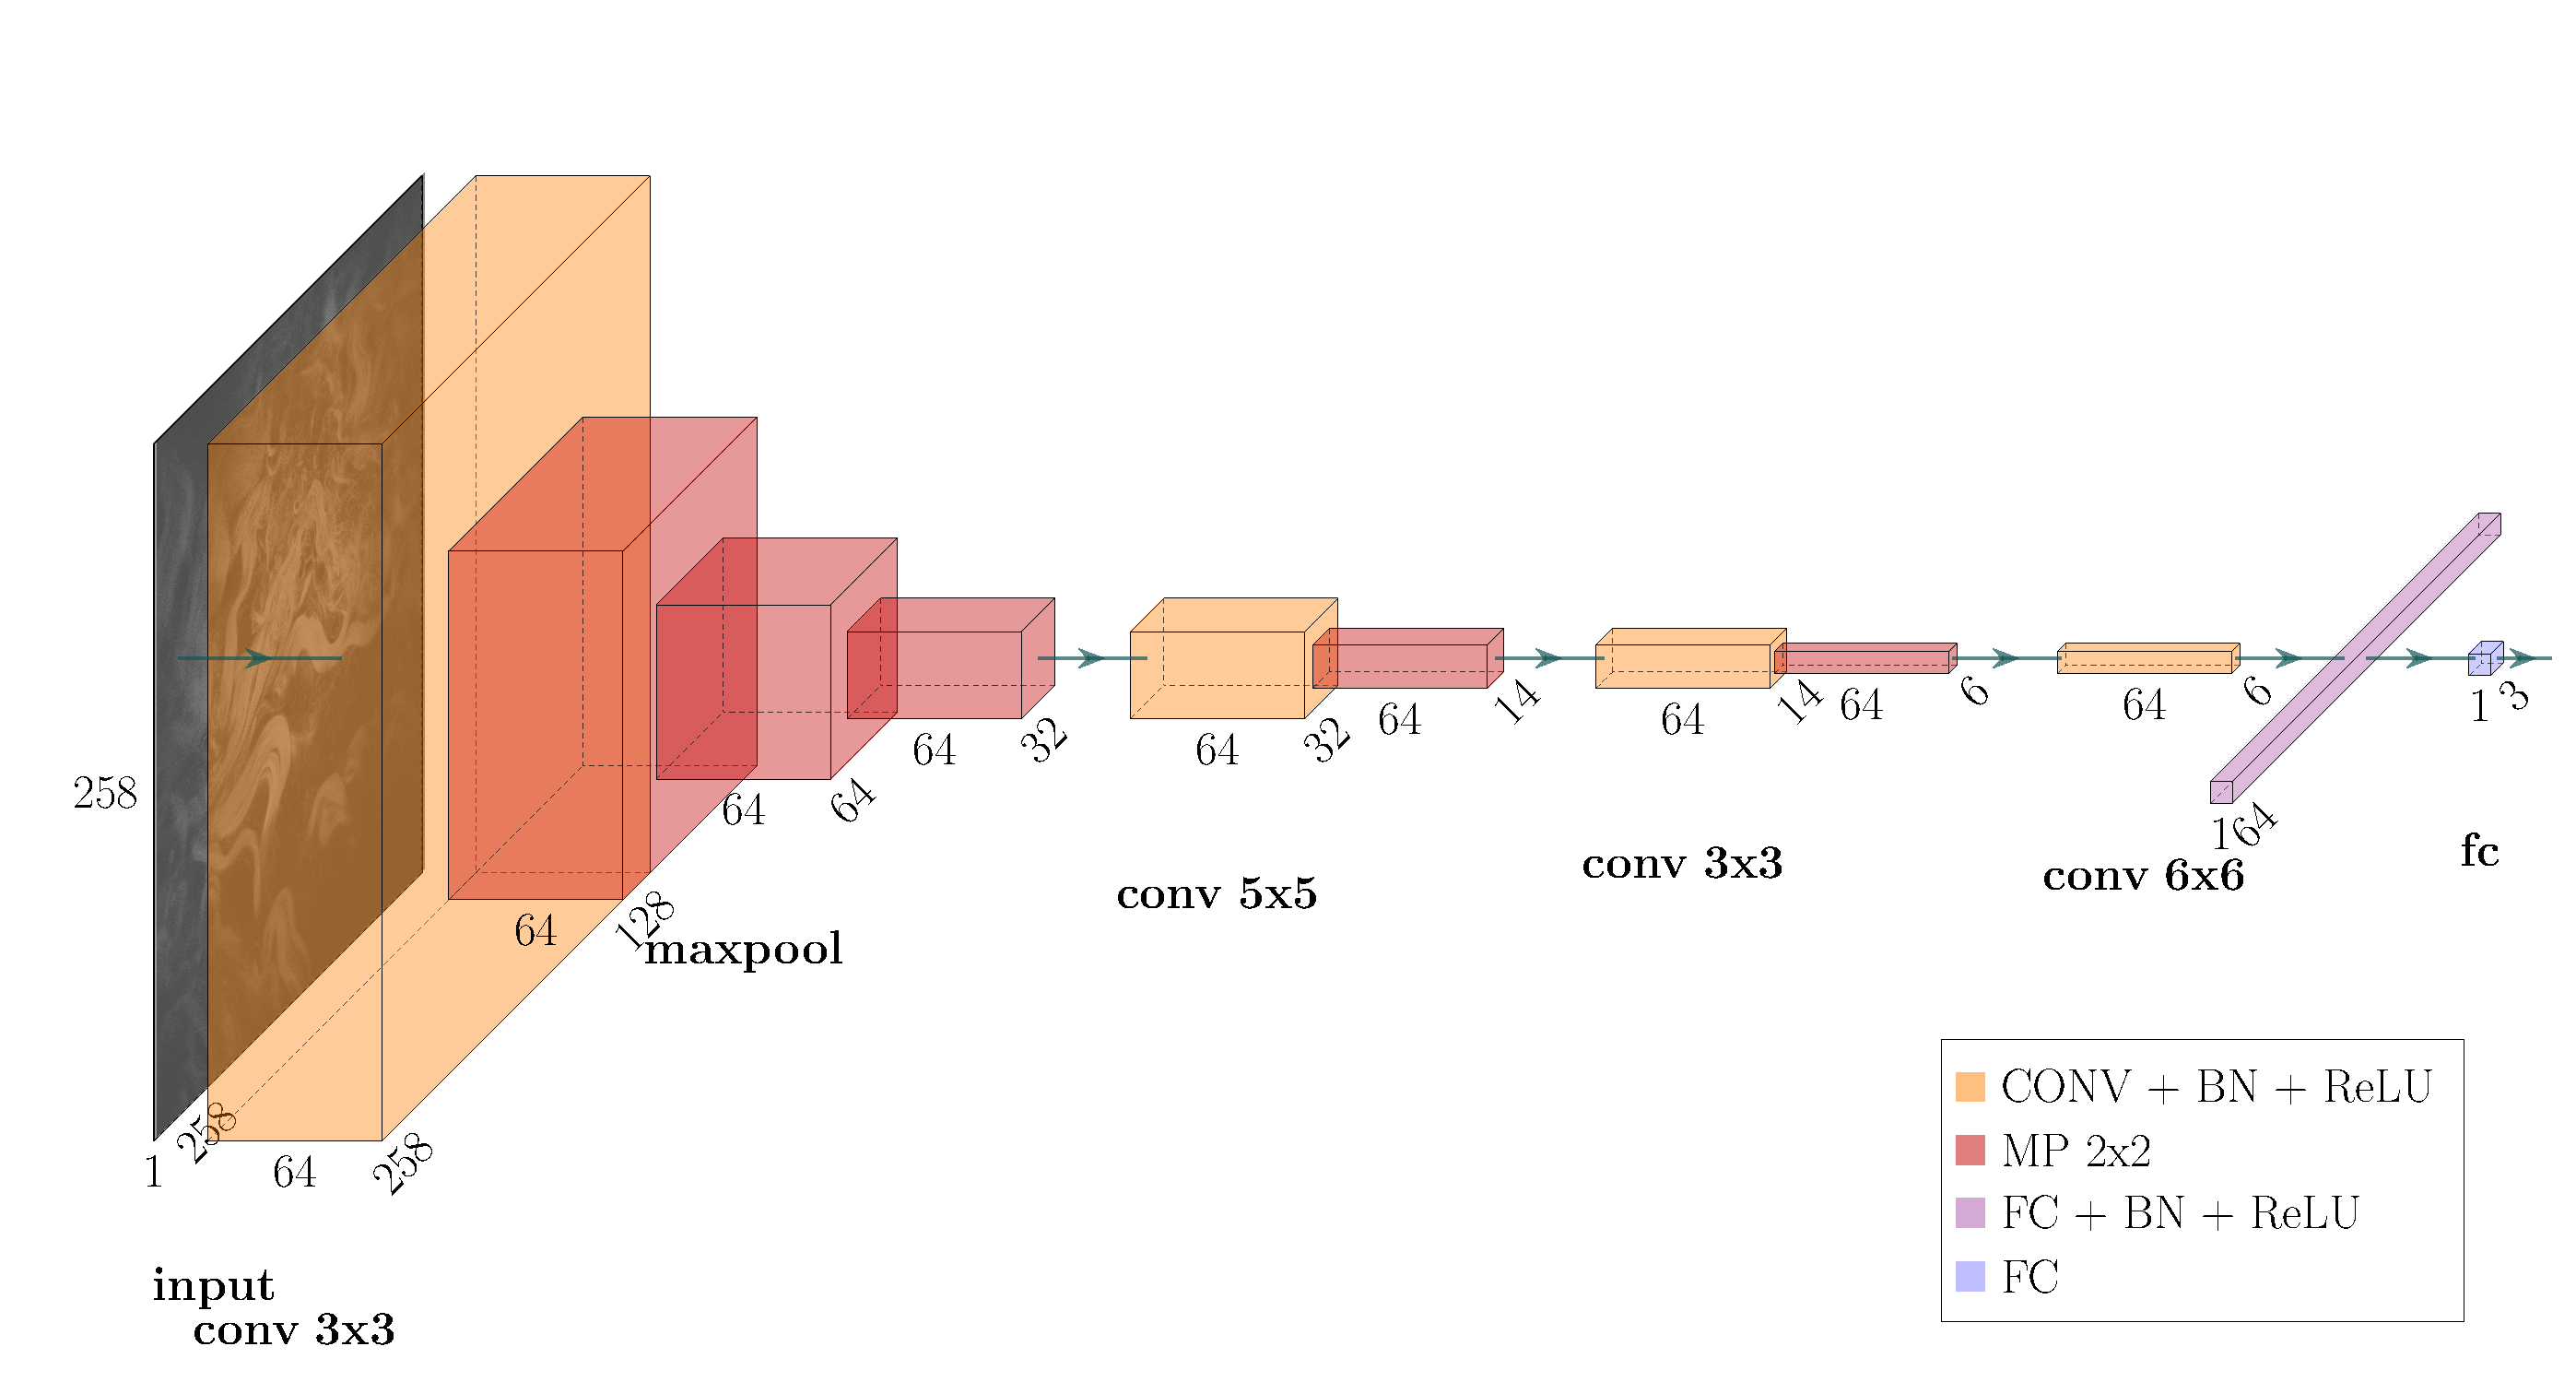
\includegraphics{skinstression/images/skinstression.pdf}
    % \input{PlotNeuralNet/examples/Skinstression/skinstression-new.tex}
    \caption[Network architecture]{
        The convolutional neural network consists of five blocks.
        The first four blocks contain convolution, maxpooling, and batch normalization layers.
        The last block contains a fully connected network.
        It requires an input of $\qty{258}{px}\times\qty{258}{px}$ to get a vector of length 3 as output.
    }
    \label{fig:model}
\end{figure*}

The dropout layers in \cite{Soylu2022} are replaced by BN layers, as the input is unnormalized and studies report better performance with BN.
Bias of all layers preceding BN layers have been set to zero.

The neural network weights are initialized according to the method described by \textcite{He2015a}, using a uniform transform.

\subsubsection{Hyperparameter optimization}
First, benchmark search 1 was done using Successive Halving with 100 trials.
See \cref{subsec:conf_skin} for a summary of configuration search space $\mathcal{C}$.
To allow trials to warmup, a minimum of 100 epochs were allowed.
To limit the trial duration, a maximum of 3000 epochs were allowed.
The number of trials were reduced with a reduction factor of $\eta=4$.
Trial parameters were sampled using the non-multivariate TPE algorithm.

The optimization was performed with the Adam optimizer ($\beta_1=0.9$, $\beta_2=0.999$), weighted focal MSE loss, and a cosine annealing with warm restarts learning rate scheduler.
Every trial used the complete dataset after data preparation (\cref{sec:skin_data_prep}).

The search uses a few data augmentations that are assumed to not alter the physical context of the image.
That is, force is exerted on the tissue in the horizontal direction in the image.
Therefore, flipping the image either vertically or horizontally is assumed to not change the stretch behaviour.
Both flipping operations occur with a probability of $0.5$.
Moreover, the images' intensity is randomly changed between x\% and x\%.\marginpar{By what fraction is the intensity changed?}

To possibly find a more optimal set of hyperparameters, two searches with the Hyperband algorithm with 300 trials was performed.
Trial parameters were sampled using the multivariate TPE algorithm.
The learning rate was warmed up linearly for the first 20 epochs.

% As shown in [ref results search 1], it seems that the network has difficulty with estimating $\gamma_c$, while $E_\mathrm{max}$ and $\sigma_\mathrm{max}$ seem to be easier estimated.
% As the original stress-strain curves do not have data in the plateau regime, $\sigma_\mathrm{max}$ was given less importance in search 2 and 3.
% This was achieved by weighting individual targets of the focal loss, such that
% \begin{equation}
%     FL = \frac{FL_{\sigma_\mathrm{max}} + FL_{E_\mathrm{max} + FL_{\gamma_c}}}{3}
% \end{equation}
% Therefore, in search 2 and 3, the goal was to give less importance to $$

Search 2 introduces random $700\times700$ cropping to further artificially increase the number of available images to train on.
% Also included is the ability to weight the loss per target variable (not to be confused with LDS), to penalize hard variables more than easy variables.
% The targets were weighted as $(\sigma_\mathrm{max},E_\mathrm{max},\gamma_c) = (0.8, 1, 1)$, to give less attention to the plateau.
Search 3 includes the Yeo-Johnson transformation to see how input normalization affects the training outcome.

For a summary of the hyperparameter searches, see \cref{tab:skin_studies}.

Algorithms provided by Optuna \cite{Akiba2019} were used to choose trial configurations and keep track of trials.

\begin{table}
    \caption[\textsc{Skinstression} hyperparameter search studies]{
        Summary of settings for hyperparameter searches performed.
        Hyperparameters are grouped by operation type (image preprocessing, image augmenting, target weighting) and in applied order.
        Every search is done with the search space described in \cref{tab:conf_skin}.
    }
    \label{tab:skin_studies}
    \begin{tabular}{lcccc}
        % \toprule
        % Search                         & 1      & 2      & 3      & 4      \\
        % \midrule
        % CLAHE                          & \cmark & \cmark & \cmark & \cmark \\
        % Yeo-Johnson transform          & \xmark & \xmark & \cmark & \xmark \\
        % \midrule
        % Random $700\times700$ cropping & \xmark & \cmark & \cmark & \cmark \\
        % Intensity jitter               & \cmark & \cmark & \cmark & \cmark \\
        % Random horizontal flip         & \cmark & \cmark & \cmark & \cmark \\
        % Random vertical flip           & \cmark & \cmark & \cmark & \cmark \\
        % Random sharpness               & \xmark & \xmark & \xmark & \cmark \\
        % Random gaussian blur           & \xmark & \xmark & \xmark & \cmark \\
        % Random rotation                & \xmark & \xmark & \xmark & \cmark \\
        % \midrule
        % Target variable weighting      & \xmark & \cmark & \cmark & \cmark \\
        % \bottomrule

        \toprule
        Search                         & 1      & 2      & 3      \\
        \midrule
        CLAHE                          & \cmark & \cmark & \cmark \\
        Yeo-Johnson transform          & \xmark & \xmark & \cmark \\
        \midrule
        Random $700\times700$ cropping & \xmark & \cmark & \cmark \\
        Intensity jitter               & \cmark & \cmark & \cmark \\
        Random horizontal flip         & \cmark & \cmark & \cmark \\
        Random vertical flip           & \cmark & \cmark & \cmark \\
        Random sharpness               & \xmark & \xmark & \xmark \\
        Random gaussian blur           & \xmark & \xmark & \xmark \\
        Random rotation                & \xmark & \xmark & \xmark \\
        % \midrule
        % Target variable weighting      & \xmark & \cmark & \cmark \\
        \midrule
        Search algorithm               & SH     & HB     & HB     \\
        Multivariate TPE               & \xmark & \cmark & \cmark \\
        trials                         & 100    & 300    & 300    \\
        learning rate warmup           & \xmark & \cmark & \cmark \\
        \bottomrule
    \end{tabular}
\end{table}

\subsubsection{Training}
Using the best configuration for hyperparameter optimization, a model is trained further for a total of 10000 epochs.
The learning rate scheduler was cosine annealing with warm restarts to allow for model ensembling later during inference (\cref{subsec:model_ensembling}), if deemed useful.
The learning rate was warmed up linearly for the first 20 epochs.
To see the influence of image quality, the model is trained using an ordered set of images.
The images are ordered with maximum entropy first and the model is trained on all images and the top 10, 20 and 30 images of every stack.
Moreover, to see the effect of using the original zoom level with the greatest detail at hand, the best 20 images of every stack were centercropped to $500\times500$ and further randomly cropped randomly to $258\times258$.
The lowest validation focal loss is used to compare model performance.
The model with the lowest validation loss is used for testing.

Pytorch \cite{Paszke2019} was used to perform automatic differentiation on NVIDIA GeForce RTX 2070 Super GPUs on the BAZIS high performance computing cluster.

\subsubsection{Dataset}\label{subsec:skin_dataset}
The thigh dataset is randomly distributed into a training (\qty{64}{\percent}), validation (\qty{16}{\percent}), and test (\qty{20}{\percent}).
The distribution is stratified by person, meaning samples corresponding to the same person cannot live in two subsets simultaneously.
The AI learns from the training set.
Every iteration, it is validated against the validation set.
During inference, the AI is applied to the test set as external validation.

% \subsubsection{Model selection}
% MISSCHIEN MODEL ENSEMBLING EN VALIDATION SET GEBRUIKEN VOOR VINDEN VAN BESTE AANTAL MODELS?
% The last $N$\marginnote{How many again?} models are ensembled together

\subsection{Explainability}

\subsubsection{Occlusion}
To explain the model output, occlusion \cref{subsec:occlusion} is used.
Using the Captum Python library \cite{Kokhlikyan2020}, occlusion is done with $3\times 3$\unit{px} square patches moving with strides of 1.
All values in the patch have been replaced with 0.

\subsubsection{Adversarial attack}
To see the importance of homogeneous tissue within the skin tissue, black patches have been filled using Fiji \cite{Schindelin2012}.
Filling is done by drawing full white ellipses on top of the original image.
Moreover, in another attack, a black patch is copied to other locations in the image.

\section{Results}

\begin{figure}
    \centering
    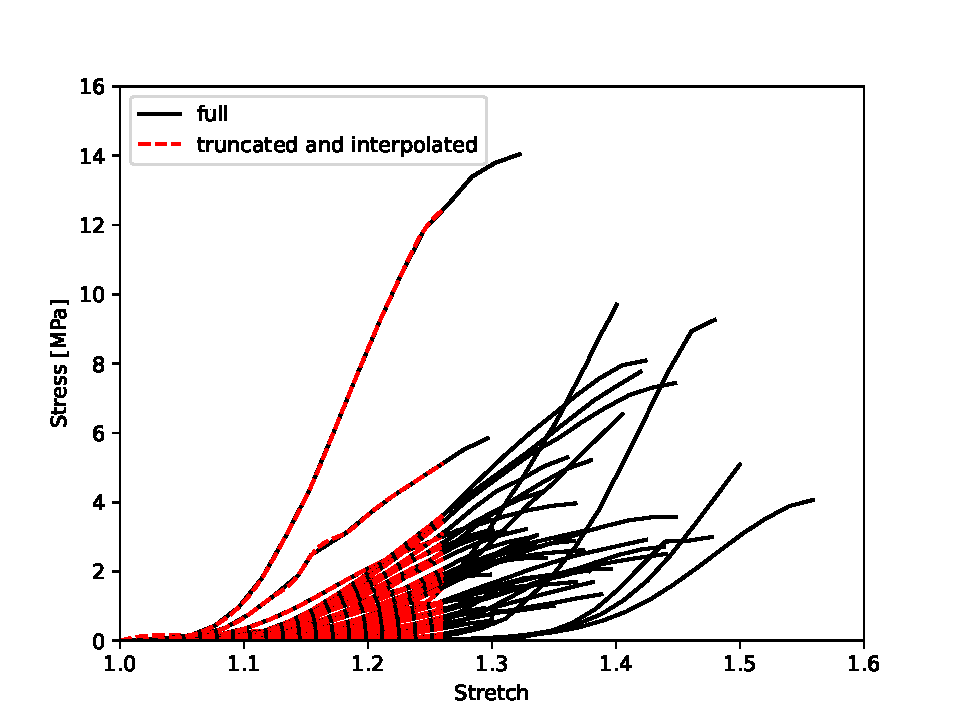
\includegraphics[width=\linewidth]{skinstression/images/truncated-and-interpolated-curves.pdf}
    \caption[Truncated and spline interpolated curves]{
        The strain-stress curves (black) were truncated and interpolated (dotted red)
        using non-uniform, interpolating splines on the stretch values of the curve with the lowest maximum stretch.
    }
    \label{fig:trunc_interp_curves}
\end{figure}

\subsection{Participants}\label{subsec:results_participants}

Earlier studies (refs) include 18 individuals (5 men, 4 women, and 6 unknown).
Abdomen data was excluded, because the strain-stress curves differ significantly from the thigh.
All thigh data is included, which is different from the original study, where only the 48 latest samples were used.
These considerations result in data including 15 individuals (5 men, 4 women, 3 unknown).
Ages range from 61 to 94.
Skin tissue is cut from the thigh and cut in multiple pieces of roughly the same shape.\marginpar{protocol?}
From every skin tissue piece, strain-stress curves are measured.
The number of measured strain-stress curves range from 1 to 13.
The source of data is summarized in \cref{fig:source_of_data}.

\begin{figure*}
    \centering
    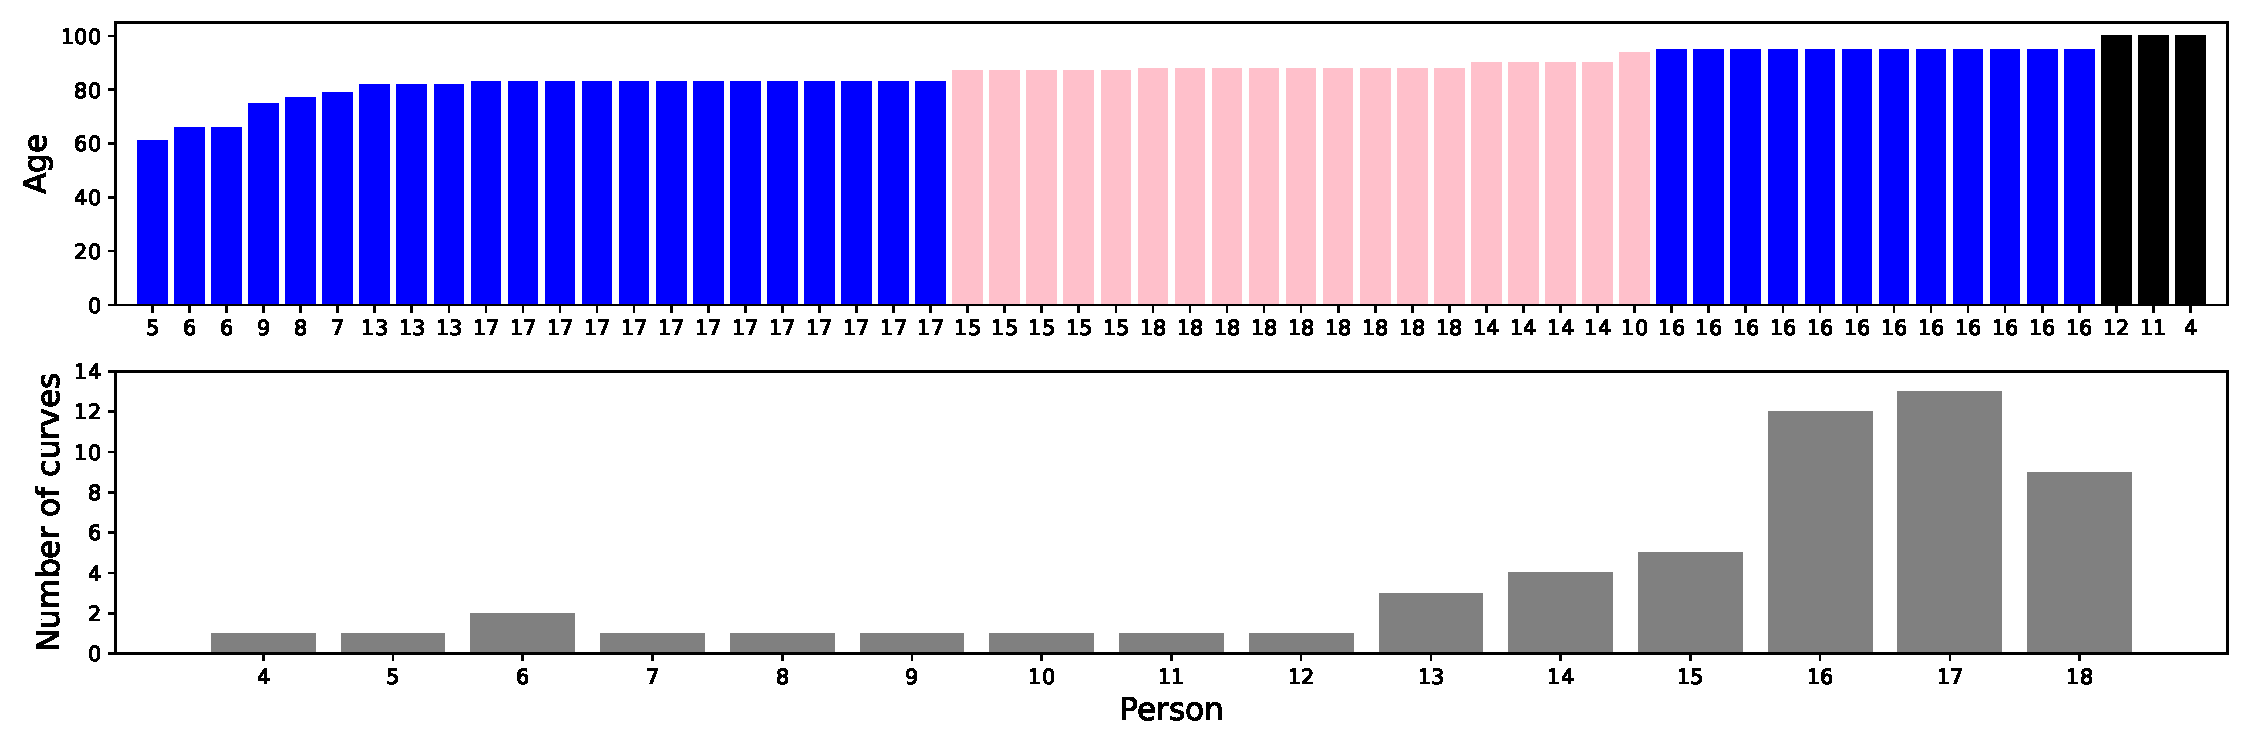
\includegraphics[width=\linewidth]{skinstression/images/age_distribution.pdf}
    \caption[Source of data]{
        The selected individuals and their sex, age and number of strain-stress curves.
        Top panel: shows the age and sex distribution. Blue, pink and black denote male, female and unknown sex.
        In fact, the age of person 12, 11, and 4 are unknown.
        Bottom panel: shows the number of curves per person.
    }
    \label{fig:source_of_data}
\end{figure*}

\subsection{Predictor pre-selection}
\subsubsection{Exponential}
An exponential fit to \cref{eq:exp} is shown in \cref{fig:exp_fits}.
$R^2 = \num{0.9497}$.
The exponent is not able to fit the plateau that is often exhibited near maximum stretch.

\begin{marginfigure}
    \centering
    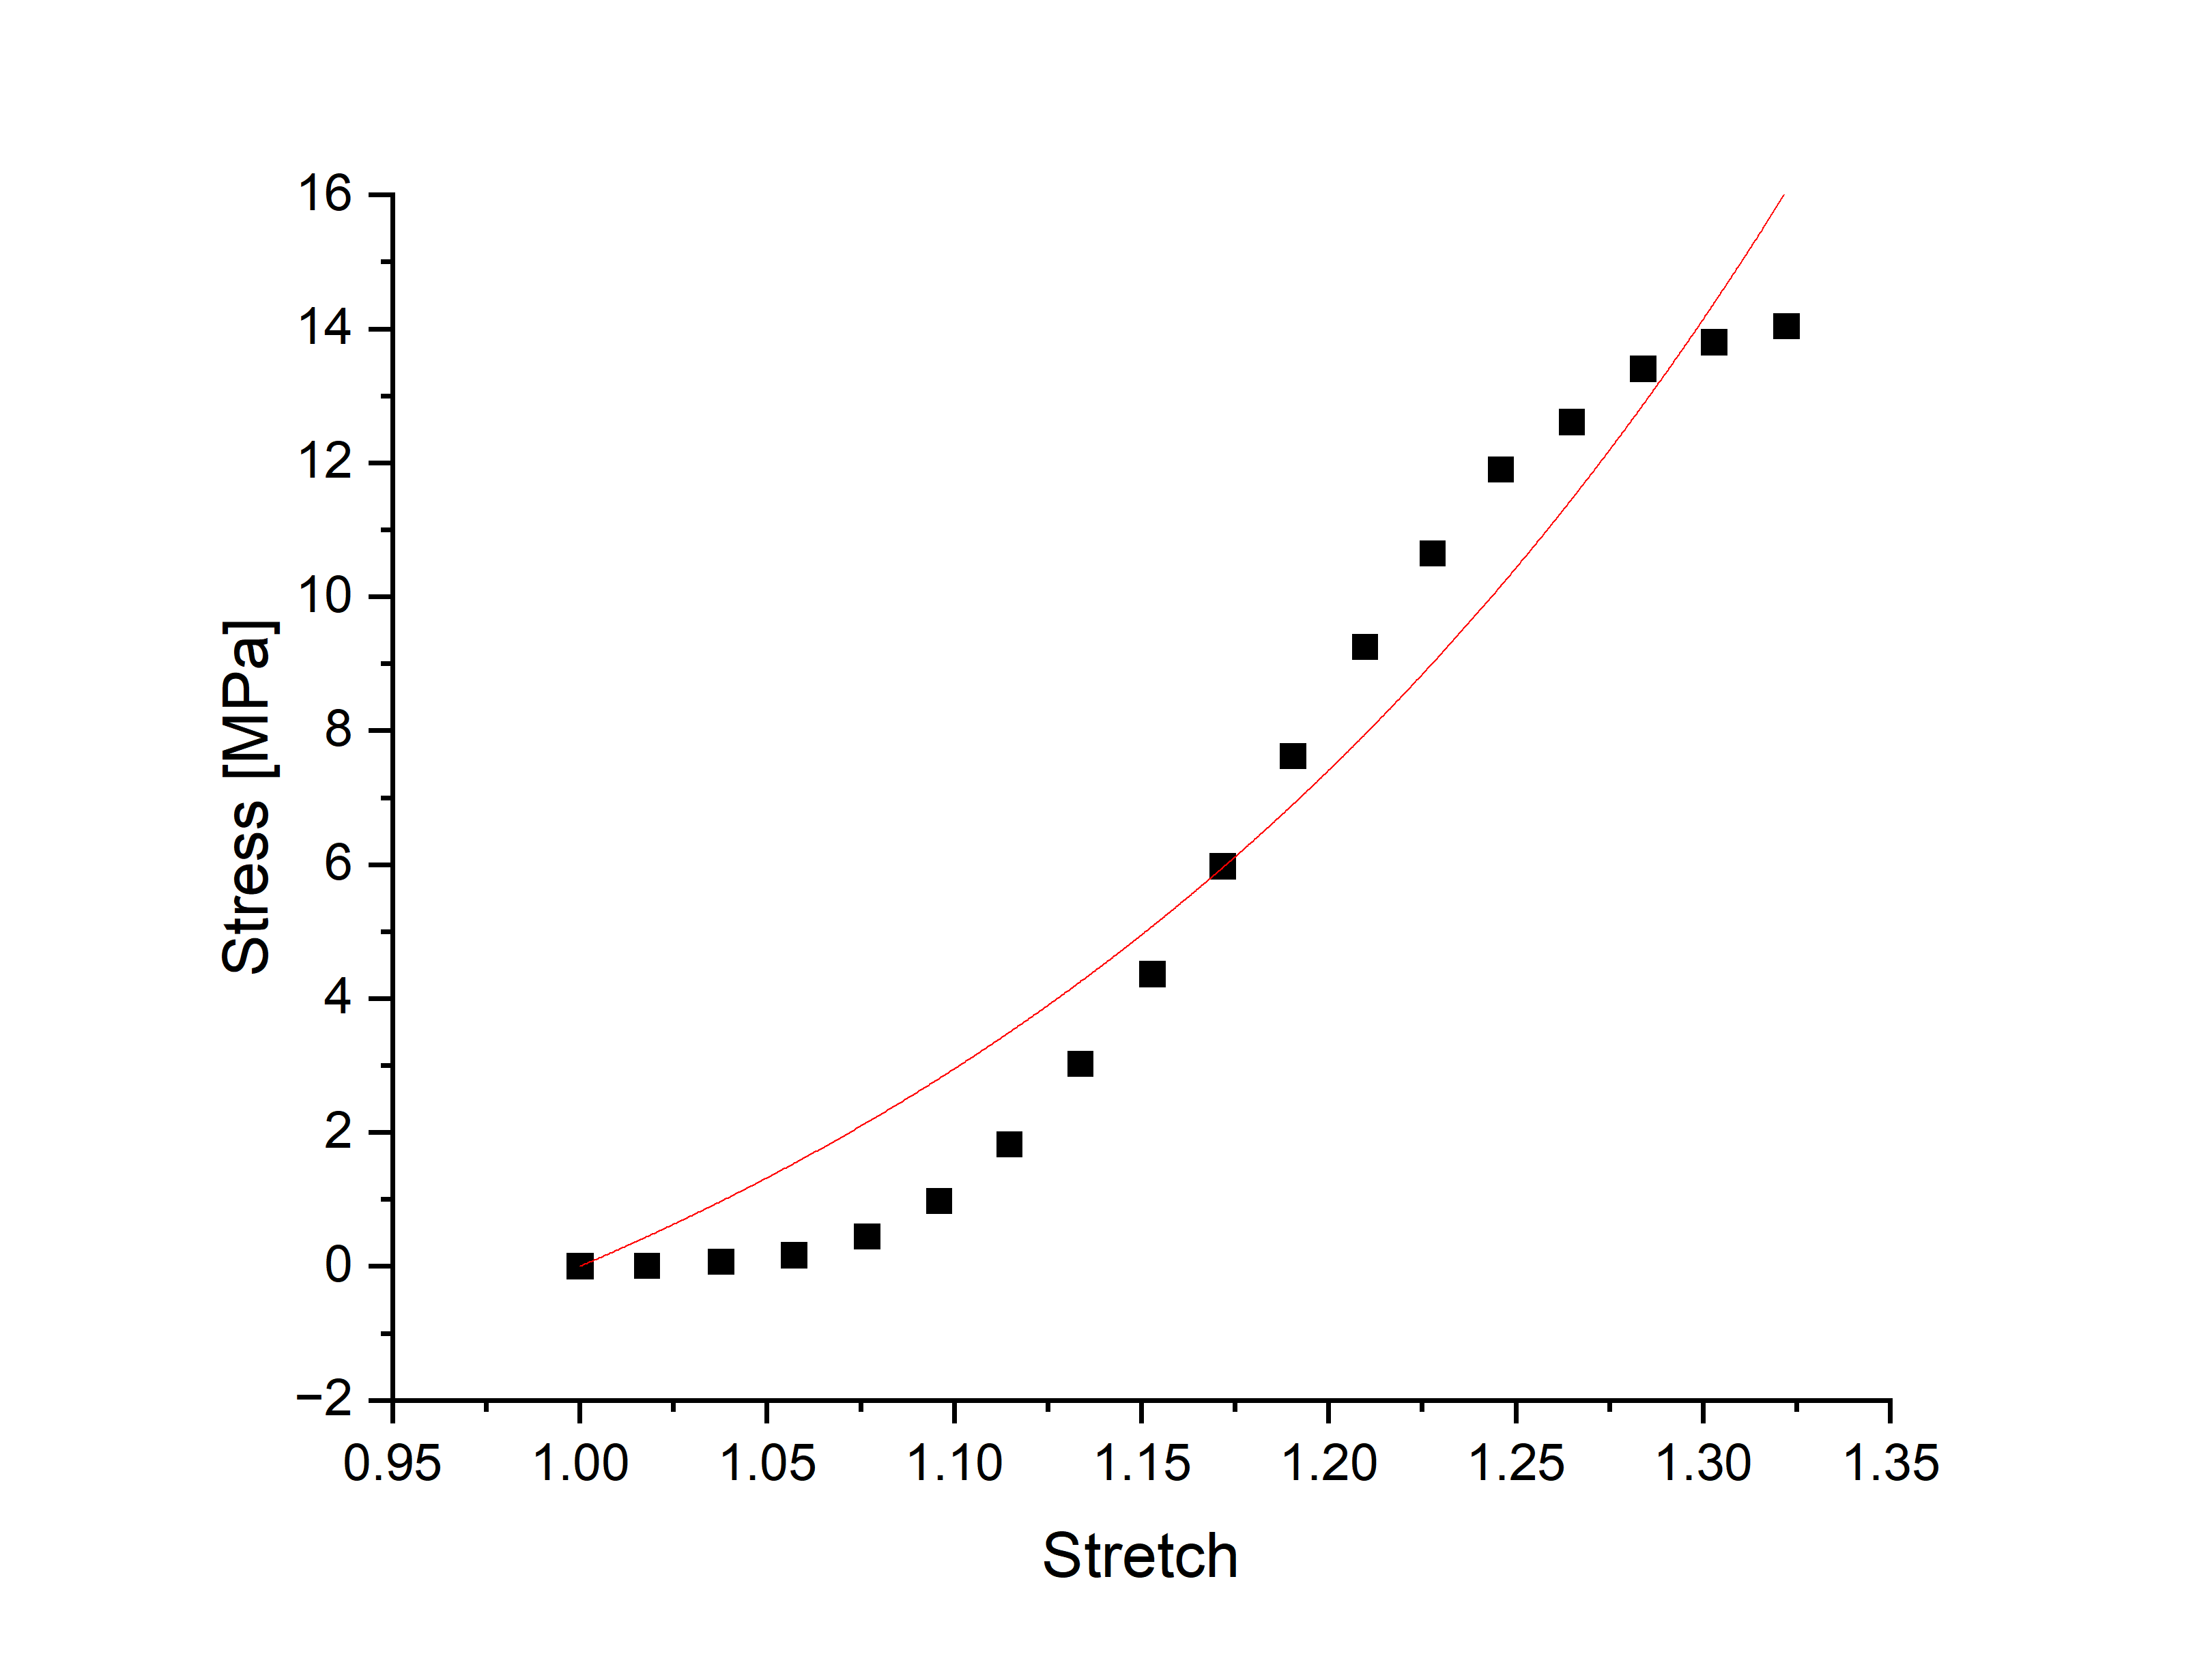
\includegraphics[width=\linewidth]{skinstression/images/exp-fits/exponential.png}
    \caption[Exponential fit]{
        Exponential fit with \cref{eq:exp} (red) for one stress-strain curve (black).
        Fit parameters were $G_0=\qty{23.8\pm4.0}{\mega\pascal\per\stretch}$, and $\lambda=\qty{4.1\pm 1.0}{\stretch}$.
        $R^2=\num{0.9497}$.
    }
    \label{fig:exp_fits}
\end{marginfigure}

\subsubsection{PCA}
The PCA fit for every truncated and interpolated strain-stress curve is depicted in \cref{fig:pca_fits}.
For every fit, $R^2$ is calculated with respect to the interpolated and truncated data.
On average, $\overline{R^2} \approx \num{0.9927 \pm 0.0022}$.
Due to the nature of PCA, the exponential part of the curves that rise later is not included in the making of the fit.

\begin{figure*}
    \ContinuedFloat
    \centering
    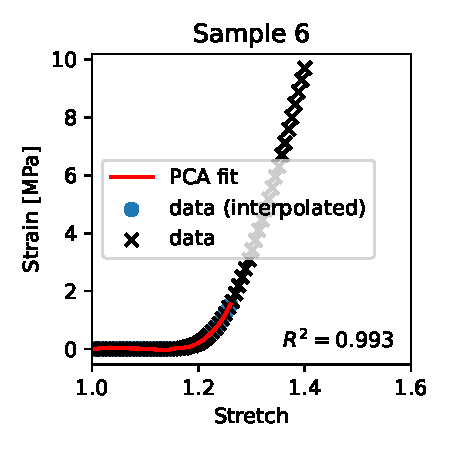
\includegraphics[width=0.24\linewidth]{skinstression/images/pca-fits/sample_6.pdf}
    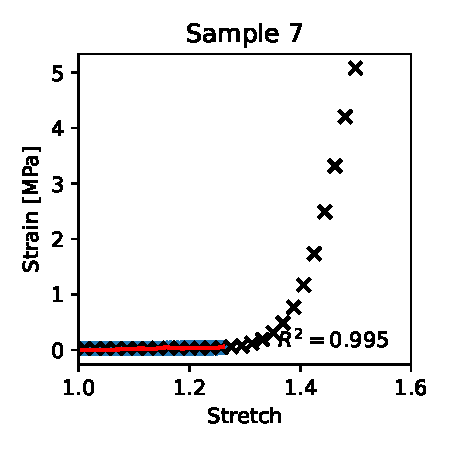
\includegraphics[width=0.24\linewidth]{skinstression/images/pca-fits/sample_7.pdf}
    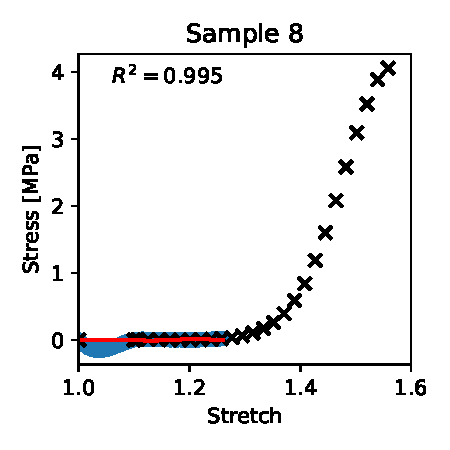
\includegraphics[width=0.24\linewidth]{skinstression/images/pca-fits/sample_8.pdf}
    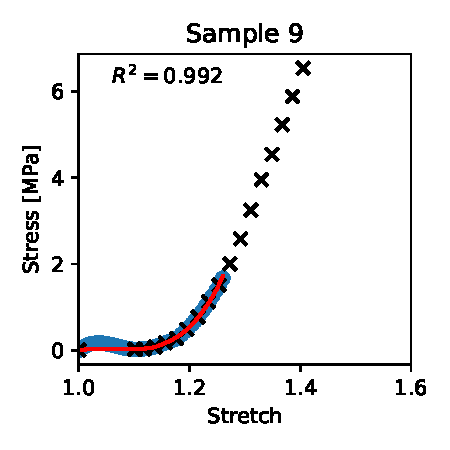
\includegraphics[width=0.24\linewidth]{skinstression/images/pca-fits/sample_9.pdf} \\
    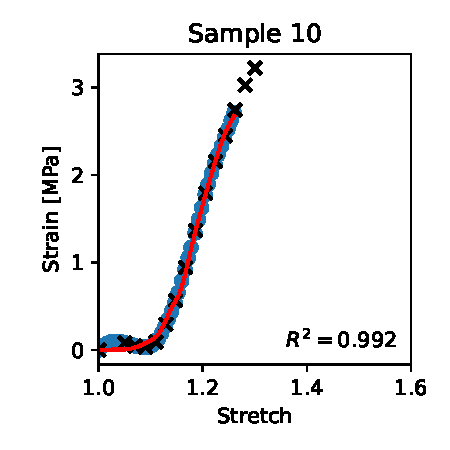
\includegraphics[width=0.24\linewidth]{skinstression/images/pca-fits/sample_10.pdf}
    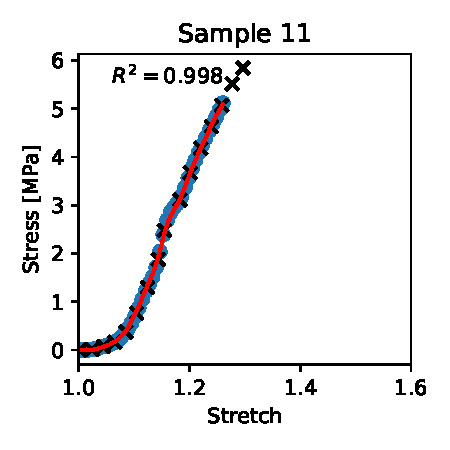
\includegraphics[width=0.24\linewidth]{skinstression/images/pca-fits/sample_11.pdf}
    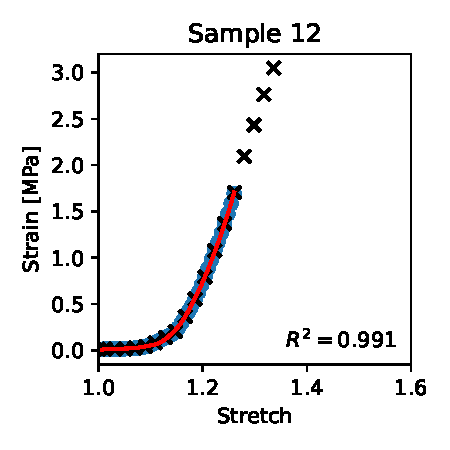
\includegraphics[width=0.24\linewidth]{skinstression/images/pca-fits/sample_12.pdf}
    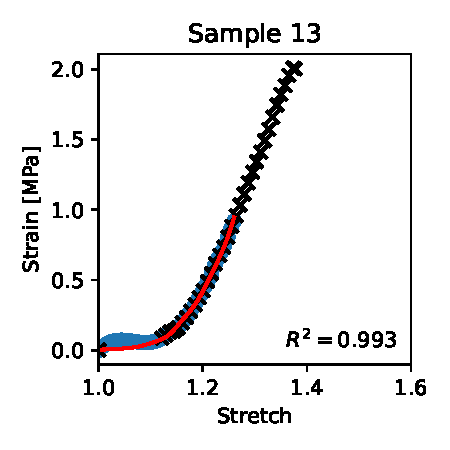
\includegraphics[width=0.24\linewidth]{skinstression/images/pca-fits/sample_13.pdf} \\
    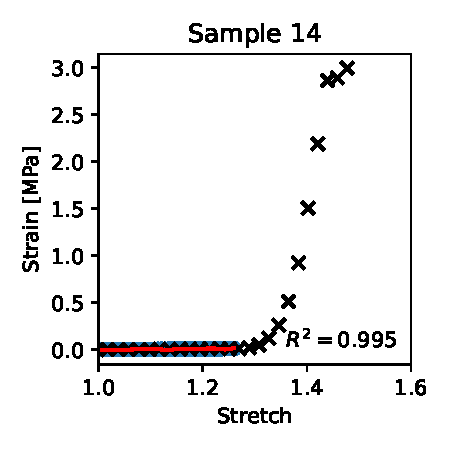
\includegraphics[width=0.24\linewidth]{skinstression/images/pca-fits/sample_14.pdf}
    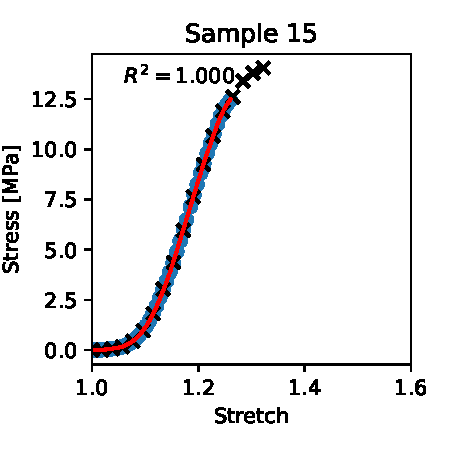
\includegraphics[width=0.24\linewidth]{skinstression/images/pca-fits/sample_15.pdf}
    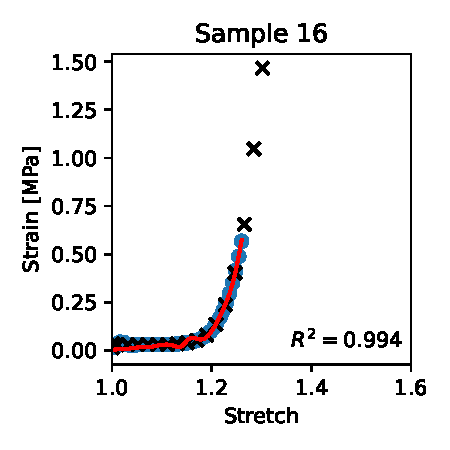
\includegraphics[width=0.24\linewidth]{skinstression/images/pca-fits/sample_16.pdf}
    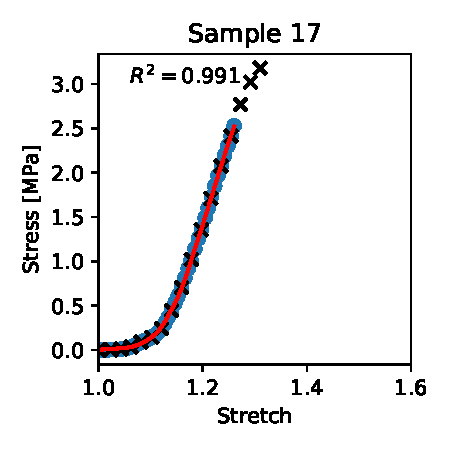
\includegraphics[width=0.24\linewidth]{skinstression/images/pca-fits/sample_17.pdf} \\
    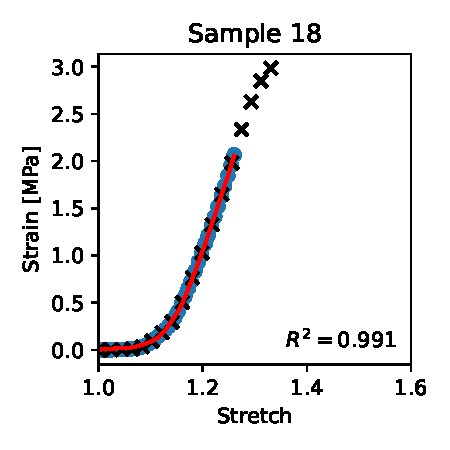
\includegraphics[width=0.24\linewidth]{skinstression/images/pca-fits/sample_18.pdf}
    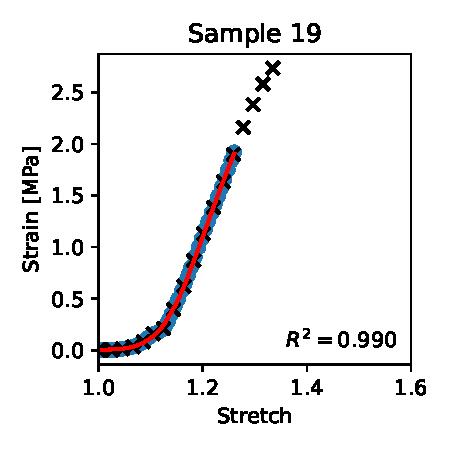
\includegraphics[width=0.24\linewidth]{skinstression/images/pca-fits/sample_19.pdf}
    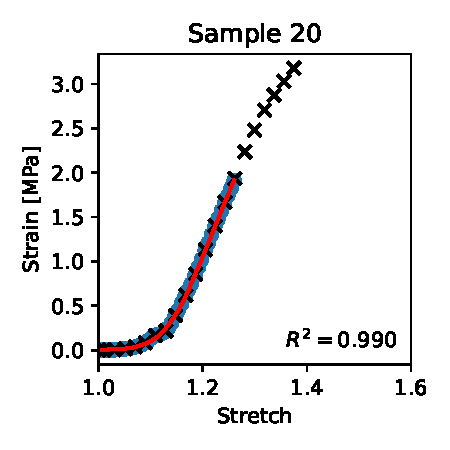
\includegraphics[width=0.24\linewidth]{skinstression/images/pca-fits/sample_20.pdf}
    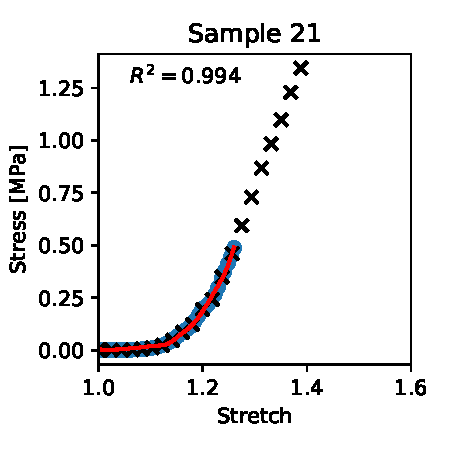
\includegraphics[width=0.24\linewidth]{skinstression/images/pca-fits/sample_21.pdf} \\
    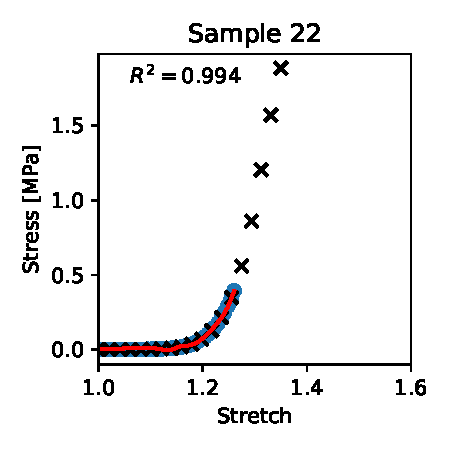
\includegraphics[width=0.24\linewidth]{skinstression/images/pca-fits/sample_22.pdf}
    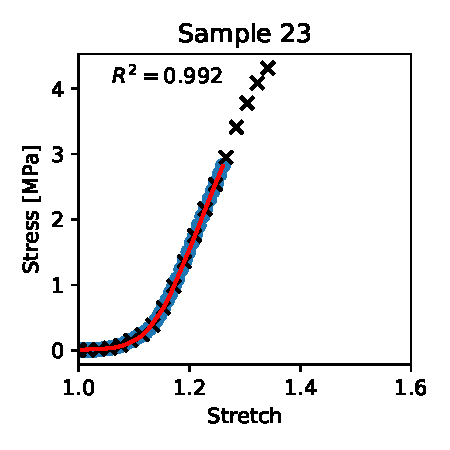
\includegraphics[width=0.24\linewidth]{skinstression/images/pca-fits/sample_23.pdf}
    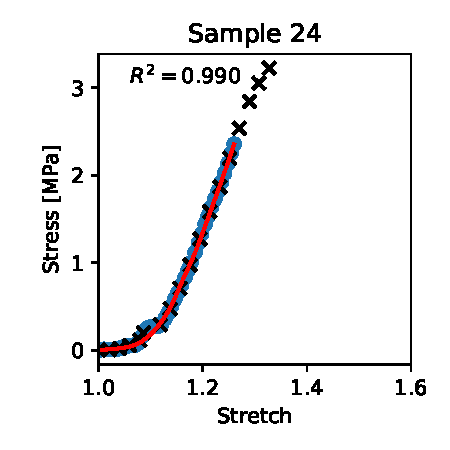
\includegraphics[width=0.24\linewidth]{skinstression/images/pca-fits/sample_24.pdf}
    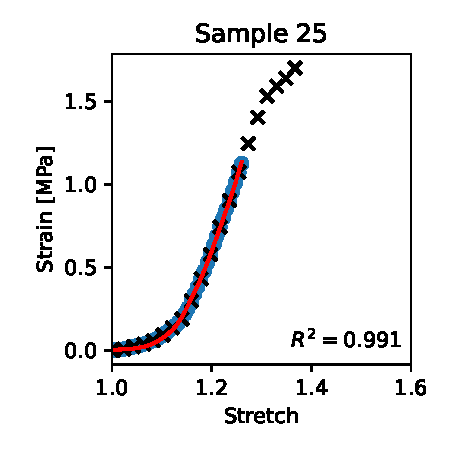
\includegraphics[width=0.24\linewidth]{skinstression/images/pca-fits/sample_25.pdf} \\
    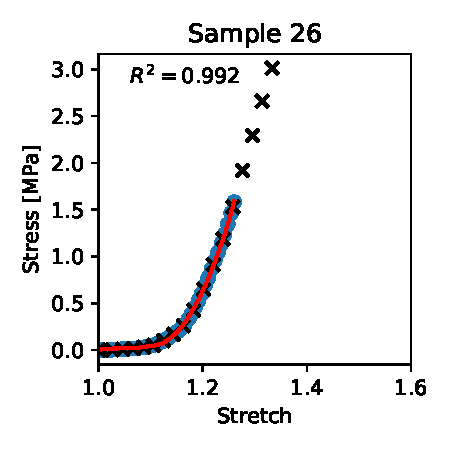
\includegraphics[width=0.24\linewidth]{skinstression/images/pca-fits/sample_26.pdf}
    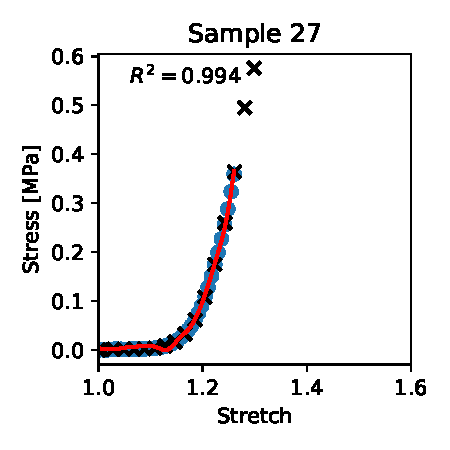
\includegraphics[width=0.24\linewidth]{skinstression/images/pca-fits/sample_27.pdf}
    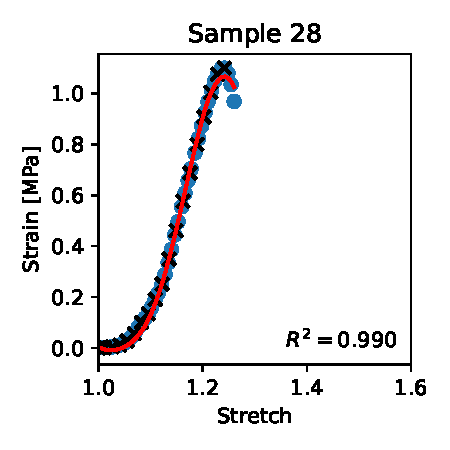
\includegraphics[width=0.24\linewidth]{skinstression/images/pca-fits/sample_28.pdf}
    \includegraphics[width=0.24\linewidth]{skinstression/images/pca-fits/sample_29.pdf}
    \raggedleft Continued on next page.
\end{figure*}

\begin{figure*}
    \centering
    \includegraphics[width=0.24\linewidth]{skinstression/images/pca-fits/sample_30.pdf}
    \includegraphics[width=0.24\linewidth]{skinstression/images/pca-fits/sample_31.pdf}
    \includegraphics[width=0.24\linewidth]{skinstression/images/pca-fits/sample_32.pdf}
    \includegraphics[width=0.24\linewidth]{skinstression/images/pca-fits/sample_33.pdf} \\
    \includegraphics[width=0.24\linewidth]{skinstression/images/pca-fits/sample_34.pdf}
    \includegraphics[width=0.24\linewidth]{skinstression/images/pca-fits/sample_45.pdf}
    \includegraphics[width=0.24\linewidth]{skinstression/images/pca-fits/sample_46.pdf}
    \includegraphics[width=0.24\linewidth]{skinstression/images/pca-fits/sample_47.pdf} \\
    \includegraphics[width=0.24\linewidth]{skinstression/images/pca-fits/sample_48.pdf}
    \includegraphics[width=0.24\linewidth]{skinstression/images/pca-fits/sample_49.pdf}
    \includegraphics[width=0.24\linewidth]{skinstression/images/pca-fits/sample_50.pdf}
    \includegraphics[width=0.24\linewidth]{skinstression/images/pca-fits/sample_51.pdf} \\
    \includegraphics[width=0.24\linewidth]{skinstression/images/pca-fits/sample_52.pdf}
    \includegraphics[width=0.24\linewidth]{skinstression/images/pca-fits/sample_53.pdf}
    \includegraphics[width=0.24\linewidth]{skinstression/images/pca-fits/sample_54.pdf}
    \includegraphics[width=0.24\linewidth]{skinstression/images/pca-fits/sample_55.pdf} \\
    \includegraphics[width=0.24\linewidth]{skinstression/images/pca-fits/sample_56.pdf}
    \includegraphics[width=0.24\linewidth]{skinstression/images/pca-fits/sample_57.pdf}
    \includegraphics[width=0.24\linewidth]{skinstression/images/pca-fits/sample_58.pdf}
    \includegraphics[width=0.24\linewidth]{skinstression/images/pca-fits/sample_59.pdf} \\
    \includegraphics[width=0.24\linewidth]{skinstression/images/pca-fits/sample_60.pdf}
    \includegraphics[width=0.24\linewidth]{skinstression/images/pca-fits/sample_61.pdf}
    \caption[PCA fits]{
        PCA fits for every truncated and interpolated strain-stress curve.
        The interpolated measurements (blue) are estimated by the PCA curve (red) along with their $R^2$.
        PCA is done on all available thigh data.
        Note that the vertical axes are not equal.
    }
    \label{fig:pca_fits}
\end{figure*}

\subsubsection{Logistic curve}
The logistic curve fit for every strain-stress curve is shown in \cref{fig:logistic_fits}.
For every fit, $R^2$ is calculated.
On average, $\overline{R^2} \approx \num{0.9979 \pm 0.0039}$.

\begin{figure*}
    \ContinuedFloat
    \centering
    \includegraphics[width=0.24\linewidth]{skinstression/images/logistic-fits/sample_6}
    \includegraphics[width=0.24\linewidth]{skinstression/images/logistic-fits/sample_7.pdf}
    \includegraphics[width=0.24\linewidth]{skinstression/images/logistic-fits/sample_8.pdf}
    \includegraphics[width=0.24\linewidth]{skinstression/images/logistic-fits/sample_9.pdf} \\
    \includegraphics[width=0.24\linewidth]{skinstression/images/logistic-fits/sample_10.pdf}
    \includegraphics[width=0.24\linewidth]{skinstression/images/logistic-fits/sample_11.pdf}
    \includegraphics[width=0.24\linewidth]{skinstression/images/logistic-fits/sample_12.pdf}
    \includegraphics[width=0.24\linewidth]{skinstression/images/logistic-fits/sample_13.pdf} \\
    \includegraphics[width=0.24\linewidth]{skinstression/images/logistic-fits/sample_14.pdf}
    \includegraphics[width=0.24\linewidth]{skinstression/images/logistic-fits/sample_15.pdf}
    \includegraphics[width=0.24\linewidth]{skinstression/images/logistic-fits/sample_16.pdf}
    \includegraphics[width=0.24\linewidth]{skinstression/images/logistic-fits/sample_17.pdf} \\
    \includegraphics[width=0.24\linewidth]{skinstression/images/logistic-fits/sample_18.pdf}
    \includegraphics[width=0.24\linewidth]{skinstression/images/logistic-fits/sample_19.pdf}
    \includegraphics[width=0.24\linewidth]{skinstression/images/logistic-fits/sample_20.pdf}
    \includegraphics[width=0.24\linewidth]{skinstression/images/logistic-fits/sample_21.pdf} \\
    \includegraphics[width=0.24\linewidth]{skinstression/images/logistic-fits/sample_22.pdf}
    \includegraphics[width=0.24\linewidth]{skinstression/images/logistic-fits/sample_23.pdf}
    \includegraphics[width=0.24\linewidth]{skinstression/images/logistic-fits/sample_24.pdf}
    \includegraphics[width=0.24\linewidth]{skinstression/images/logistic-fits/sample_25.pdf} \\
    \includegraphics[width=0.24\linewidth]{skinstression/images/logistic-fits/sample_26.pdf}
    \includegraphics[width=0.24\linewidth]{skinstression/images/logistic-fits/sample_27.pdf}
    \includegraphics[width=0.24\linewidth]{skinstression/images/logistic-fits/sample_28.pdf}
    \includegraphics[width=0.24\linewidth]{skinstression/images/logistic-fits/sample_29.pdf}
    \raggedleft Continued on next page.
\end{figure*}

\begin{figure*}
    \centering
    \includegraphics[width=0.24\linewidth]{skinstression/images/logistic-fits/sample_30.pdf}
    \includegraphics[width=0.24\linewidth]{skinstression/images/logistic-fits/sample_31.pdf}
    \includegraphics[width=0.24\linewidth]{skinstression/images/logistic-fits/sample_32.pdf}
    \includegraphics[width=0.24\linewidth]{skinstression/images/logistic-fits/sample_33.pdf} \\
    \includegraphics[width=0.24\linewidth]{skinstression/images/logistic-fits/sample_34.pdf}
    \includegraphics[width=0.24\linewidth]{skinstression/images/logistic-fits/sample_45.pdf}
    \includegraphics[width=0.24\linewidth]{skinstression/images/logistic-fits/sample_46.pdf}
    \includegraphics[width=0.24\linewidth]{skinstression/images/logistic-fits/sample_47.pdf} \\
    \includegraphics[width=0.24\linewidth]{skinstression/images/logistic-fits/sample_48.pdf}
    \includegraphics[width=0.24\linewidth]{skinstression/images/logistic-fits/sample_49.pdf}
    \includegraphics[width=0.24\linewidth]{skinstression/images/logistic-fits/sample_50.pdf}
    \includegraphics[width=0.24\linewidth]{skinstression/images/logistic-fits/sample_51.pdf} \\
    \includegraphics[width=0.24\linewidth]{skinstression/images/logistic-fits/sample_52.pdf}
    \includegraphics[width=0.24\linewidth]{skinstression/images/logistic-fits/sample_53.pdf}
    \includegraphics[width=0.24\linewidth]{skinstression/images/logistic-fits/sample_54.pdf}
    \includegraphics[width=0.24\linewidth]{skinstression/images/logistic-fits/sample_55.pdf} \\
    \includegraphics[width=0.24\linewidth]{skinstression/images/logistic-fits/sample_56.pdf}
    \includegraphics[width=0.24\linewidth]{skinstression/images/logistic-fits/sample_57.pdf}
    \includegraphics[width=0.24\linewidth]{skinstression/images/logistic-fits/sample_58.pdf}
    \includegraphics[width=0.24\linewidth]{skinstression/images/logistic-fits/sample_59.pdf} \\
    \includegraphics[width=0.24\linewidth]{skinstression/images/logistic-fits/sample_60.pdf}
    \includegraphics[width=0.24\linewidth]{skinstression/images/logistic-fits/sample_61.pdf}
    \caption[Logistic fits]{
        Logistic fits (red) and their $R^2$ for every strain-stress curve (black).
        Note that the vertical axes are not equal.
    }
    \label{fig:logistic_fits}
\end{figure*}

Because the logistic curve describes the stress-strain data more accurate than PCA or the exponential, it will be used from now on.

\subsubsection{Label density smoothing}
The labels were smoothed using LDS using gaussian kernels.
All kernels had a size of 30 and a standard deviation of 3.
The distribution bins were manually set to $(\sigma_{\mathrm{max},\mathrm{min}}, \sigma_{\mathrm{max},\mathrm{max}}, s_{\sigma_\mathrm{max}}) = (0, 15, 0.01) \unit{\mega\pascal}$,
$(E_{\mathrm{max},\mathrm{min}}, E_{\mathrm{max},\mathrm{max}}, s_{E_\mathrm{max}}) = (0, 50, 0.1) \unit{\mega\pascal\per\stretch}$, and
$(\gamma_{c,\mathrm{min}}, \gamma_{\mathrm{max},\mathrm{max}}, s_{\gamma_\mathrm{max}}) = (1, 1.5, 0.001) \unit{\stretch}$,
where $s$ is the bin width.
The smoothed distribution is shown in \cref{fig:skin_lds}.

\begin{figure*}
    \centering
    \includegraphics{skinstression/images/lds/a.pdf} \\
    \includegraphics{skinstression/images/lds/k.pdf} \\
    \includegraphics{skinstression/images/lds/xc.pdf}
    \caption[Original target and LDS distrutions]{
        Empirical target distribution (red) and LDS distribution (blue) for $\sigma_\mathrm{max}$, $E_\mathrm{max}$, and $\gamma_c$.
        LDS aims to fill the gaps between the actual measurements.
        LDS also extrapolates target distributions.
        For all targets, the kernel size was 30 units, and the standard deviation 3 units.
        The bin width were \num{0.01}, \num{0.1}, and \num{0.001} units for $\sigma_\mathrm{max}$, $E_\mathrm{max}$, and $\gamma_c$, respectively.
    }
    \label{fig:skin_lds}
\end{figure*}

%%%%%%%%%%%%%%%%%%%%%%%%%%%%
% IMAGE QUALITY
%%%%%%%%%%%%%%%%%%%%%%%%%%%%

\subsection{Image quality}
Presumably, the model will yield erroneous predictions if images of bad quality are provided.
Moreover, the measurement was not always done in the same order, \ie from the lowest to the highest tissue or vice versa.
Therefore, two image quality measurements were explored: Shannon entropy and kurtosis.

The kurtosis of some image stacks were used to validate the image quality by eye, see \cref{fig:skin_kurtosis_depth}.
The entropy of the same image stacks as for kurtosis were used to validate the image quality by eye, see \cref{fig:skin_entropy_depth}.

For reasons explained in \cref{sec:disc_ent_vs_kur}, entropy is further used to choose the top quality images from every stack.

\begin{figure*}
    \centering
    \includegraphics[width=\linewidth]{skinstression/images/kurtosis/8.pdf} \\
    % \includegraphics[width=\linewidth]{skinstression/images/kurtosis/9.pdf} \\
    \includegraphics[width=\linewidth]{skinstression/images/kurtosis/11.pdf} \\
    \includegraphics[width=\linewidth]{skinstression/images/kurtosis/22.pdf} \\
    \includegraphics[width=\linewidth]{skinstression/images/kurtosis/27.pdf} \\
    % \includegraphics[width=\linewidth]{skinstression/images/kurtosis/28.pdf} \\
    \includegraphics[width=\linewidth]{skinstression/images/kurtosis/37.pdf}
    \caption[Kurtosis vs image stack depth]{
        Kurtosis as a function of image stack depth for a representing subset.
        Four images which are equally spaced in physical units are inset.
    }
    \label{fig:skin_kurtosis_depth}
\end{figure*}

\begin{figure*}
    \centering
    \includegraphics[width=\linewidth]{skinstression/images/entropy/8.pdf} \\
    % \includegraphics[width=\linewidth]{skinstression/images/entropy/9.pdf} \\
    \includegraphics[width=\linewidth]{skinstression/images/entropy/11.pdf} \\
    \includegraphics[width=\linewidth]{skinstression/images/entropy/22.pdf} \\
    \includegraphics[width=\linewidth]{skinstression/images/entropy/27.pdf} \\
    % \includegraphics[width=\linewidth]{skinstression/images/entropy/28.pdf} \\
    \includegraphics[width=\linewidth]{skinstression/images/entropy/37.pdf}
    \caption[Shannon entropy vs image stack depth]{
        Normalized Shannon entropy as a function of image stack depth for a representing subset.
        Four images which are equally spaced in physical units are inset.
    }
    \label{fig:skin_entropy_depth}
\end{figure*}

%%%%%%%%%%%%%%%%%%%%%%%%%%%%%%%%%%%%
% HYPERPARAMETER SEARCH
%%%%%%%%%%%%%%%%%%%%%%%%%%%%%%%%%%%%

\subsection{Hyperparameter optimization}

The loss curves of the best trials of every search are shown in \cref{fig:skinstression-search-best-loss}
Both training and validation loss show an increase at the learning rate restarts.

\begin{figure*}
    \centering
    \includegraphics[width=0.33\linewidth]{skinstression/images/hyperparameter-search/search-1/best-trial-loss.pdf}
    \includegraphics[width=0.33\linewidth]{skinstression/images/hyperparameter-search/search-2/best-trial-loss.pdf}
    \includegraphics[width=0.33\linewidth]{skinstression/images/hyperparameter-search/search-3/best-trial-loss.pdf}
    \caption[Hyperparameter search best losses]{
        Successive halving trial 71 of 100 has shown the best loss for search 1.
        Hyperband trial 184 of 300 has shown the best loss for search 2.
        Hyperband trial 73 of 300 has shown the best loss for search 3.
        The training loss (black) and validation loss (light green) are shown.
        The learning rate (orange) restarts explain sudden increase in loss.
    }
    \label{fig:skinstression-search-best-loss}
\end{figure*}

% \subsubsection{Search 1}
% The contour plot is shown in \cref{fig:skinstression-search1-contour}.
% Only the loss curves of the best trial (71) is shown in \cref{fig:skinstression-search1-best-loss}.
% Both training and validation loss show an increase at the learning rate restarts.

% \begin{figure}
%     \centering
%     \includegraphics[]{skinstression/images/hyperparameter-search/search-1/best-trial-loss.pdf}
%     \caption[Best loss curve of search 1]{
%         Successive halving trial 71 of 100 has shown the best loss for search 1.
%         The training loss (black) is followed by the validation loss (light green).
%         The learning rate (orange) restarts explain sudden increase in loss.
%     }
%     \label{fig:skinstression-search1-best-loss}
% \end{figure}

% \begin{figure*}
%     \centering
%     \includegraphics[width=\linewidth]{skinstression/images/hyperparameter-search/search-1/contour.pdf}
%     % \includegraphics[angle=90,width=0.9\textheight, height=\linewidth,keepaspectratio]{skinstression/images/hyperparameter-search/search-1/contour.pdf}
%     \caption[Search 1 contour plot]{
%         Contour plot of search 1.
%         Darker regions denote better results.
%         This contour plot is only constructed from trials which have not been pruned.
%     }
%     \label{fig:skinstression-search1-contour}
% \end{figure*}

% \subsubsection{Search 2}
% The contour plot is shown in \cref{fig:skinstression-search2-contour}.
% Only the loss curves of the best trial (184) is shown in \cref{fig:skinstression-search2-best-loss}.
% Both training and validation loss show an increase at the learning rate restarts.

% \begin{figure}
%     \centering
%     \includegraphics[]{skinstression/images/hyperparameter-search/search-2/best-trial-loss.pdf}
%     \caption[Best loss curve of search 2]{
%         Hyperband trial 184 of 300 has shown the best loss for search 2.
%         The training loss (black) is followed by the validation loss (light green).
%         The learning rate (orange) restarts explain sudden increase in loss.
%     }
%     \label{fig:skinstression-search2-best-loss}
% \end{figure}

% \begin{figure*}
%     \includegraphics[angle=90,width=0.9\textheight, height=\linewidth,keepaspectratio]{skinstression/images/hyperparameter-search/search-2/contour.pdf}
%     \caption[Search 2 contour plot]{
%         Contour plot of search 2.
%         Darker regions denote better results.
%         This contour plot is only constructed from trials which have not been pruned.
%     }
%     \label{fig:skinstression-search2-contour}
% \end{figure*}

% \subsubsection{Search 3}
% The contour plot is shown in \cref{fig:skinstression-search3-contour}.
% Only the loss curves of the best trial (73) is shown in \cref{fig:skinstression-search3-best-loss}.
% The training and validation losses diverge, showing the model overfits.

% \begin{figure}
%     \centering
%     \includegraphics[]{skinstression/images/hyperparameter-search/search-3/best-trial-loss.pdf}
%     \caption[Best loss curve of search 3]{
%         Hyperband trial 73 of 300 has shown the best loss for search 3.
%         The training loss (black) and the validation loss (light green) diverge.
%         The learning rate (orange).
%         The trial was pruned at epoch 100.
%     }
%     \label{fig:skinstression-search3-best-loss}
% \end{figure}

% \begin{figure*}
%     \centering
%     \includegraphics[angle=90,width=0.9\textheight, height=\linewidth,keepaspectratio]{skinstression/images/hyperparameter-search/search-3/contour.pdf}
%     \caption[Search 3 contour plot]{
%         Contour plot of search 3.
%         Darker regions denote better results.
%         This contour plot is only constructed from trials which have not been pruned.
%     }
%     \label{fig:skinstression-search3-contour}
% \end{figure*}

%%%%%%%%%%%%%%%%%%
% TRAINING
%%%%%%%%%%%%%%%%%%
\subsection{Training}
Training was done on the best performing set of hyperparameters, which was found by search 1.
Search 1 yielded the lowest validation loss.
The corresponding hyperparameters in \cref{tab:conf_skin_final} were used for further training.

\begin{margintable}
    \centering
    \caption[\textsc{Skinstression} configuration]{
        \textsc{Skinstression} configuration used during training.
        Parameters are ordered by their importance, calculated with fANOVA.
        LR, WD, and BS are learning rate, weight decay and batch size, respectively.
    }
    \label{tab:conf_skin_final}
    \begin{tabular}{l c c c c c c}
        \toprule
        Param.               & Value         & Imp. \\
        \midrule
        {LR}                 & 0.00747       & 0.41 \\
        {$T_0$}              & 145           & 0.24 \\
        {WD}                 & \num{2.97e-5} & 0.22 \\
        {$n_\mathrm{nodes}$} & 64            & 0.08 \\
        {$T_\mathrm{mult}$}  & 2             & 0.05 \\
        {BS}                 & 16            & 0.00 \\
        \bottomrule
    \end{tabular}
\end{margintable}

Three trainings were performed.
For every training, the 10, 20, and 30 images of every stack with highest entropy were selected to exclude any noisy images.
Also, using the 20 best images of every stack, the model is trained without scaling of the original image.
The loss curves are shown in \cref{fig:skinstression-training}.
The lowest validation losses are shown in \cref{tab:skin_train_102030}.
Overall, the model trained with 20 images shows the lowest total loss.
This model will be used during testing.

To verify performance of training, the stress-strain curves of a random training batch are plotted with the raw data in \cref{fig:skinstression-train-logistic-curves}.
For this batch, $\overline{R^2} = \num{0.75 \pm 0.28}$ with a \qty{95}{\percent} confidence interval.


\begin{figure*}
    \centering
    \includegraphics[width=0.48\linewidth]{skinstression/images/training/Training_10_images.pdf}
    \includegraphics[width=0.48\linewidth]{skinstression/images/training/Training_20_images.pdf} \\
    \includegraphics[width=0.48\linewidth]{skinstression/images/training/Training_30_images.pdf}
    \includegraphics[width=0.48\linewidth]{skinstression/images/training/Training_at_1X_zoom.pdf}
    \caption[Training losses]{
        Training losses when using 10, 20, and 30 images as well as a training using 20 images, but with unscaled images.
        The training loss (black) is followed by the validation loss (light green).
        The learning rate (orange) restarts explain sudden increase in loss.
    }
    \label{fig:skinstression-training}
\end{figure*}

\begin{margintable}
    \centering
    \caption[Lowest validation loss per $N_\mathrm{best}$ images]{
        Lowest validation loss per $N_\mathrm{best}$ images.
        The training using 20 images has the lowest validation loss.
        * denotes training without rescaling.
    }
    \label{tab:skin_train_102030}
    \begin{tabular}{S[table-align-text-post=false, table-format=3.0] S[table-format=1.4]}
        \toprule
        {\# Images}  & {Validation loss} \\
        \midrule
        10           & 0.0097            \\
        \bfseries 20 & \bfseries 0.0035  \\
        20*          & 0.27              \\
        30           & 0.0040            \\
        \bottomrule
    \end{tabular}
\end{margintable}

\begin{figure*}
    \centering
    \includegraphics[width=0.24\linewidth]{skinstression/images/training/sample_6_0.pdf}
    \includegraphics[width=0.24\linewidth]{skinstression/images/training/sample_10_0.pdf}
    \includegraphics[width=0.24\linewidth]{skinstression/images/training/sample_12_0.pdf}
    \includegraphics[width=0.24\linewidth]{skinstression/images/training/sample_15_0.pdf} \\
    \includegraphics[width=0.24\linewidth]{skinstression/images/training/sample_16_0.pdf}
    \includegraphics[width=0.24\linewidth]{skinstression/images/training/sample_18_0.pdf}
    \includegraphics[width=0.24\linewidth]{skinstression/images/training/sample_19_0.pdf}
    \includegraphics[width=0.24\linewidth]{skinstression/images/training/sample_28_0.pdf} \\
    \includegraphics[width=0.24\linewidth]{skinstression/images/training/sample_30_0.pdf}
    \includegraphics[width=0.24\linewidth]{skinstression/images/training/sample_32_0.pdf}
    \includegraphics[width=0.24\linewidth]{skinstression/images/training/sample_35_0.pdf}
    \includegraphics[width=0.24\linewidth]{skinstression/images/training/sample_37_0.pdf} \\
    \includegraphics[width=0.24\linewidth]{skinstression/images/training/sample_44_1.pdf}
    \includegraphics[width=0.24\linewidth]{skinstression/images/training/sample_46_0.pdf}
    \caption[Training results]{
        Results of a random training batch.
        Raw mechanical measurement without error bars ($\times$) are shown together with the AI fit (red).
        Performance is quantified by $R^2$.
    }
    \label{fig:skinstression-train-logistic-curves}
\end{figure*}

\subsection{Testing}
The results of the best performing images in the test set are shown in \cref{fig:skinstression-test}.
The higher $R^2$, the better the performance.
Over the best performing images of every sample, a low $\overline{R^2} = \num{-0.36 \pm 1.3}$ with a \qty{95}{\percent} confidence interval.

The performance difference between the training and test set is significant.
The donors of the test set are both male and female with ages comparable to the training set (see \cref{subsec:results_participants}).
However, most samples of the test set originate from the same person.
If the skin of this donor exhibits other behaviour, it might be difficult for the AI to predict well.

\begin{figure*}
    \centering
    \includegraphics[width=0.24\linewidth]{skinstression/images/testing/sample_51_11.pdf}
    \includegraphics[width=0.24\linewidth]{skinstression/images/testing/sample_52_15.pdf}
    \includegraphics[width=0.24\linewidth]{skinstression/images/testing/sample_53_12.pdf}
    \includegraphics[width=0.24\linewidth]{skinstression/images/testing/sample_54_17.pdf} \\
    \includegraphics[width=0.24\linewidth]{skinstression/images/testing/sample_55_10.pdf}
    \includegraphics[width=0.24\linewidth]{skinstression/images/testing/sample_56_9.pdf}
    \includegraphics[width=0.24\linewidth]{skinstression/images/testing/sample_57_19.pdf}
    \includegraphics[width=0.24\linewidth]{skinstression/images/testing/sample_58_17.pdf} \\
    \includegraphics[width=0.24\linewidth]{skinstression/images/testing/sample_59_16.pdf}
    \includegraphics[width=0.24\linewidth]{skinstression/images/testing/sample_60_10.pdf}
    \includegraphics[width=0.24\linewidth]{skinstression/images/testing/sample_61_18.pdf}
    \caption[Test results]{
        Results of the best performing image per sample are shown.
        Performance is quantified by $R^2$.
    }
    \label{fig:skinstression-test}
\end{figure*}

\subsection{Model specification}
The foundational neural network is described in \cref{fig:model}.
x neural networks combined make up the final model.
The output of the model is the average of the outputs of the individual models.
It accepts a batch of images as input and outputs a vector $(i, \sigma_\mathrm{max}, E_\mathrm{max}, \gamma_c)$,
where $i$ denotes the $i$th image of the batch.

\subsection{Usability}
The prediction AI may be used for two purposes.
One purpose is to skip the mechanical measurement on skin tissue and immediately get an estimation of stretch properties.
Another is to match stretch information to physical features present in the collagen fiber networks.
The model should not be used as validation for the mechanical measurement, as it is trained and tested on a dataset with small variance.

Input data should be assessed on quality.
A measure of quality is Shannon entropy, which is used in this study.
However, the model may benefit from other quality measures.
The user should experiment what measure works best.
The application does allow to only select the top $N_\mathrm{best}$ images.

The model only accepts batches of two-dimensional $500x500\,\unit{px}$ images.
Currently, the user should separate any higher-dimensional data and crop the images to fit the model.

\subsection{Explainability}

\subsubsection{Occlusion}
Algorithmically occluded images have been presented to the model to obtain attributions at the pixel level.
For a summary of the test set, they are shown in blended heatmaps in \cref{fig:skin_occlusion}.
\cref{fig:skin_occlusion_53} shows attribution maps for all test images of sample 53.

Attributions appear to coincide with collagen fibers.
This is important, as the abundance of collagen is hypothesized to relate to the stretch properties.
It is unclear how positive and negative attributions give insight into the prediction of stretch properties.
It is important to note that attribution maps belonging to the best performing predictions give the most appropriate insight into the AI reasoning.

The heatmaps give limited insight into the performance errors between samples across the test set or images within a sample.
There is no clear relation between the attribution mean and/or standard deviation and $R^2$.

% \begin{figure*}
%     \ContinuedFloat
%     \centering
%     \includegraphics[width=\linewidth]{skinstression/images/explainability/occlusion/0.pdf} \\
%     \raggedleft Continued on next page.
% \end{figure*}
\begin{figure*}
    % \ContinuedFloat
    \centering
    \includegraphics[width=\linewidth]{skinstression/images/explainability/occlusion/summary_test_0.pdf}
    \caption[Original image and attribution heat maps]{
        Original image and attribution heat maps.
        Attributions are blended with the original image.
        Attributions were calculated using $20\times 20\unit{px}$ occlusion.
        Color scale is from \numrange{-3}{3} units, and is linear from \qtyrange{-0.1}{0.1}{\mega\pascal}, \qtyrange{-0.1}{0.1}{\mega\pascal\per\stretch}, and \qtyrange{-0.001}{0.001}{\stretch}.
        Mean $\pm$ standard deviation are inset.
        Zoom in in the digital version for details.
    }
    \label{fig:skin_occlusion}
\end{figure*}


\begin{figure*}
    \ContinuedFloat
    \centering
    \includegraphics[width=\linewidth]{skinstression/images/explainability/occlusion/summary_53_0.pdf} \\
    \raggedleft Continued on next page.
\end{figure*}
\begin{figure*}
    % \ContinuedFloat
    \centering
    \includegraphics[width=\linewidth]{skinstression/images/explainability/occlusion/summary_53_1.pdf}
    \caption[Original image and attribution heat maps for sample 53]{
        Original image and attribution heat maps for sample 53.
        Attributions are blended with the original image.
        Attributions were calculated using $20\times 20\unit{px}$ occlusion.
        Green and red show which parts attribute to under- and overestimations, compared to output calculated from an unoccluded image.
        Color scale is from \numrange{-1.5}{1.5} units, and is linear from \qtyrange{-0.1}{0.1}{\mega\pascal}, \qtyrange{-0.1}{0.1}{\mega\pascal\per\stretch}, and \qtyrange{-0.001}{0.001}{\stretch}.
        Mean $\pm$ standard deviation are inset.
        Zoom in in the digital version for details.
    }
    \label{fig:skin_occlusion_53}
\end{figure*}

\subsubsection{Adversarial attack}
\Cref{fig:attack_occlusion} shows attribution maps for all outputs to compare attacked images with the original image.
\Cref{fig:pred_output_attack} shows the predicted logistic curves for the attacked images and the original image.
These results show that artificially filling holes increases the stiffness and resistance, while adding holes decreases stiffness and resistance.

\begin{figure*}
    \centering
    \includegraphics[width=\linewidth]{skinstression/images/attack/attack-viz.pdf} \\
    \includegraphics[width=\linewidth]{skinstression/images/attack/holes-occlusion-0.pdf} \\
    \includegraphics[width=\linewidth]{skinstression/images/attack/holes-occlusion-1.pdf} \\
    \includegraphics[width=\linewidth]{skinstression/images/attack/holes-occlusion-2.pdf}
    \caption[Occlusion on attacked image]{
        Top row shows a visualization of the two attacks.
        The middle image has holes filled with white.
        The right image has duplicates of one hole.
        The next rows show occlusion attribution maps for all outputs.
        Color scales are equal to \cref{fig:skin_occlusion_53}.
    }
    \label{fig:attack_occlusion}
\end{figure*}

\begin{figure}
    \centering
    \includegraphics{skinstression/images/attack/holes.pdf}
    \caption[Prediction output after hole attack]{
        Prediction output after hole attack.
    }
    \label{fig:pred_output_attack}
\end{figure}
\section{Discussion}

TODO?:
\begin{enumerate}
    \item collagen is viscoelastic and is therefore timedependent.
    \item discard strain-stress curve outliers (using PCA?)
    \item (random cropping has a higher probability of including pixels in the middle region)
    \item WHY DEEP LEARNING?
    \item train/val/test diff of 'source of data' fig
\end{enumerate}

\subsection{Logistic curve fits stress-strain curves better than an exponential or PCA}
With an $\overline{R^2} \approx \num{0.9979 \pm 0.0039}$, the logistic curve fits stress-strain data (\cref{fig:logistic_fits}) better than the exponential or PCA ($\overline{R^2} \approx \num{0.9927 \pm 0.0022}$, \cref{fig:pca_fits}).
The exponential does not fit the plateau that is often present at the end of a stress-strain curve (\cref{fig:exp_fits}).
This plateau is essential to the skin tissue dynamics.
It shows at which point the integrity of the collagen matrix breaks down, \ie when the skin cannot resist the force acting on it.
PCA had to be done after truncating all curves to maximum strain of the curve with the smallest maximum strain.
This resulted in PCA fits that only described the first region of the curve.
Moreover, to fairly create PCA fits, PCA has to be trained on a training set and values extracted from the test set must be projected onto this test set.
This may lead to generalizability problems.
For these reasons, the logistic curve parameters are used as a predictors.

\subsection{Shannon entropy is a better measure to exclude noise than kurtosis}\label{sec:disc_ent_vs_kur}
Measures to be used to exclude noise are kurtosis (\cref{fig:skin_kurtosis_depth}) and Shannon entropy (\cref{fig:skin_entropy_depth}).
For rather homogeneous images like stack 8, kurtosis is able to characterize the fogginess, while entropy finds images of equal quality.
However, for well-structured tissue like stack 11, 12, 13 and 4, entropy recognizes faint images and qualifies them as bad.
This is particularly useful for images that did not include any useful information (like stack 37).
Kurtosis does not succeed to distinguish dark images from bright ones.
Kurtosis also has the tendency to fluctuate, which is unexpected between subsequent slices.
For these reasons, Shannon entropy has been used to choose the top $N_\mathrm{best}$ images.

\subsection{Stretch information can be extracted from SHG microscopy images}
\Cref{fig:skinstression-train-logistic-curves} shows that for most images, it is possible to extract stretch information.
Using the model, ten images from different stacks of the train set yield a stress-strain curve with $R^2>0.9$.
This shows that stretch information is present, even in the drastically downsized images.

\subsection{The model does not generalize well}
Although the train results were promising, the test results of \cref{fig:skinstression-test} show a lack of generalizability.
Only two images from different stacks of the test set yield a stress-strain curve with $R^2=0.99$.
This shows that the training set does not include enough features similar to the features in the test set.
More images need to be included in the training set for the model to generalize well to held-out test cases.

\subsection{Artificially increasing collagen density increases maximum stress prediction and stiffness and vice versa}
As shown in \cref{fig:pred_output_attack}, artificially filling holes with collagen increases the maximum stress significantly and increases the maximum Young's modulus slightly.
This is expected, as an increase in collagen density generally is an increase in the number of springs in the system.
Adding springs increases the stiffness.
The increase in maximum stress is likely due to the addition of springs supporting each other dividing the load.
On the contrary, with comparable reasoning, artificially decreasing the collagen density by duplicating a hole lowers both the maximum stress and Young's modulus.

\subsection{Future studies}
\subsubsection{Perform cross validation and increase data variance}
In this study, no cross validation is performed.
Training a network on different training subsets might increase the performance on the test set.
The test set might include patterns that were not present in the training set and therefore will not activate critical parts of the neural network.
The split between training and test sets should be made such that the training set has high variance and is thus a reasonably good estimate of the whole population, without knowing test set images.

Therefore, the training set should also include images from human skin that is damaged in any way.
For example, damaged tissue is caused by smoking \cite{Lipa2021} or wounds that left behind scars with an increased tensile strength \cite{Wilkinson2020}.
Moreover, aging drastically impacts skin tissue integrity.
It is unknown if stretch of young skin tissue is predicted well by the neural network.
Therefore, the neural network should only be used to predict from old skin tissue.

Skin tissue from other body parts might show different stretch properties.
Therefore, it is unknown if the stretch of skin tissues other than from the upper leg can be predicted.

Lastly, to increase variance, more images of skin tissue from more individuals should be included.

\subsubsection{Split dataset before image and target transformations}
LDS should only be performed on the training set, independently from the validation and test set.
This is to prevent leaking data to the training set.
By design, the software constructs train, validation and test split datasets with data transformations, including target transformations such as LDS and the Yeo-Johnson transformation.
Every split in fact contains all $N_\mathrm{best}$ images and includes transformations.
Just before constructing a dataloader, the datasets are split by index, leaving the dataloaders with non-overlapping data.
In future studies, the dataset should be split into subsets with their specific transformations applied.
While this increases training fairness, it is expected to decrease performance, as information from the test set is not leaked to the training set.

Moreover, the split indices were generated by shuffling $\{1,\, 2,\, 3,\, \ldots,\, N_\mathrm{images}\}$ and splitting the indices at \qty{80}{\percent}, giving indices for the training/validation and test set.
Next, a new set of indices, $\{1,\, 2,\, 3,\, \ldots,\, \qty{80}{\percent} \cdot N_\mathrm{images}\}$ is shuffled and split at \qty{80}{\percent}, yielding indices for the training and validation set.
All splits were stratified by person, meaning the shuffle was done in such a way that images from the same person could not live in the training or validation set.
This way, the training and validation set had overlap with the test set, but not with each other.
To create an independent test set, the operation
\begin{equation}\label{eq:skin_newtest_idx}
    \texttt{actual test} = \texttt{test} - (\texttt{train} \cup \texttt{validation})
\end{equation}
was performed.
However, this does not make use of the full dataset.
To achieve that, \cref{eq:skin_newtest_idx} should be rewritten as
\begin{equation}
    \texttt{actual test} = \{1,\, 2,\, 3,\, \ldots,\, N_\mathrm{images}\} - (\texttt{train} \cup \texttt{validation}).
\end{equation}
This version of \texttt{actual test} has one major drawback, which is that the \qty{20}{\percent} highest indices are reserved for the test set, effectively excluding them from the shuffle.
A future study should perform a train/validation split on shuffled indices after splitting off the test set.

\subsubsection{Excluding noise and denoising on stack level}
Currently, the stacks are truncated by taking the top $N_\mathrm{best}$ images of a stack which effectively excludes noisy slices.
However, if a full z-stack is noisy, noisy images are still included.
These noisy images may still harm training and could be excluded, too.
Possibly, excluding noisy stacks can for example be done by calculating the Shannon entropy of all truncated stacks and include stacks with the highest entropy.

In addition to noise exclusion, denoising stacks with three-dimensional N2V or individual slices with N2V2\footnote{At the time of writing, N2V2 is not yet compatible with three-dimensional images.} could increase model performance.
This is because noise can occlude patterns that describe stretch information.

\subsubsection{Using three-dimensional images}
The current model relies on single images belonging to stacks.
All structural information in the depth direction is disregarded by the neural network.
If the neural network is redesigned to recognize patterns in three dimensions, it is expected to better predict the skin stretch properties.

\subsubsection{Using full-size images}
The microscope outputting the SHG images has the ability to image with a resolution of \qty{0.2}{\micro\meter}, which is five times higher than the images used in this study.
Higher resolution images contain more detailed information on the collagen structure, and are therefore expected to increase the performance.
The presented model has to be redesigned to accept images larger than $258\times258$.
Moreover, raw data is stored with a larger dynamic range (16-bit instead of 8-bit).
Being able to see small differences in neighbouring pixel intensities increases the available information \eg in darker regions, where collagen is sparse, but still significantly present.

\subsubsection{Weighting samples by goodness of target fit}
The neural network learns from targets that are a result of logistic curves fitted to a series of datapoints.
The goodness of fit differs between curves.
Fits that do not describe the data well should not negatively impact the model training.
One way to achieve this is by reweighting the loss function as
\begin{equation}
    \mathcal{L}_{R^2\,\mathrm{weighted}} =
    \begin{cases}
        \mathcal{L} / \left(R^2\right)^b & \text{if } R^2 > a     \\
        \mathcal{L} / a^b                & \text{if } R^2 \leq a,
    \end{cases}
\end{equation}
where $a$ is a lower bound to $R^2$ and $b > 0$ can influence the amount of weighting.

\subsection{Implications}
\subsubsection{Clinical \emph{in vivo} skin studies}
An example of clinical use could ultimately be to study skin tissue \emph{in vivo} by a plastic surgeon with a microendoscope as described by \textcite{Kuzmin2016}, but for SHG imaging.
Stretch information could be inferred directly from the images made by the microendoscope.
This way, the surgeon can acquire specific patient skin information prior to surgery.
It is important to note that the model in its current form has low predictive accuracy, and needs further research for this use case.
\section{Supplementary materials}
\subsection{Code}
The implementation of Skinstression can be found at \href{https://github.io/siemdejong/shg-strain-stress}{\faIcon{github} siemdejong/shg-strain-stress}.
The context and container diagram are depicted in \cref{app:skin_c4}.

\subsection{Data}
(Is the data available somewhere online?
Did Mengyao publish it with her research and can I refer to it?)

\pagelayout{wide} % No margins
\chapter{Pediatric brain tumours}
\pagelayout{margin} % Restore margins

\subsection{Multi-instance learning}

Now that a SimCLR trained backbone is trained and tiles can be compressed into feature vectors, the features can be used for classification.
To this end, a classifier must be chosen and trained.
Multi-instance learning (MIL) is a suitable technique to deal with multiple features concerning the same outcome.

\subsubsection{Classical}
Multi-instance learning (MIL) is a supervised learning method.
Typically, every instance in a dataset is labelled individually.
However, with MIL, the model receives a bag of instances, $B=\{(x_1,y_1),\ldots,(x_K,y_K)\}$, where $x$ is an instance with label $y$.
Under the standard assumption, the label of a bag is
\begin{align}
    Y(B) &= 1 - \prod_{k}^{K}(1-y_k) \\
         &= \max_k(y_k),
\end{align}
\ie, a bag is positive if at least one instance is positive.

The standard assumption is asymmetric: the meaning of the bag label changes if positive and negative labels are swapped.
This assumption might be too restrictive in non-binary problems.

See \cref{fig:classifier} for a schematic overview of a general MIL model.

\begin{figure*}
    \centering
    \includesvg[width=\linewidth]{pediatric-brain-tumours/images/classifier.svg}
    \caption[Multi-instance learning classification]{
        Extracted features (tile features in this work) are presented to a multi-layer perceptron (MLP) with learnable weights.
        The first MLP outputs an aggregate that summarizes all input features.
        The aggregate is used as input to a classifier MLP with learnable weights that outputs a prediction.
        Weights are updated based on pre-defined loss between prediction and target.
    }
    \label{fig:classifier}
\end{figure*}

\subsubsection{Attention-based MIL pooling}
For pathology studies, it is important to visualize which instances are important for classification.
With classical MIL, this is not possible.
To overcome the restrictive nature of maximum pooling, \citeauthor{Ilse2018} \sidecite{Ilse2018} propose DeepMIL and use an adaptive weighted average of instances.
This weighted average includes learnable weights in an attention-based manner.
High weights should be assigned to instances that are likely to have a positive label.
The weights allow distinguishing interesting instances from uninteresting ones, see \cref{fig:explainer}.
The attention weights of specific instances (\eg, patches in an image) explain how the model comes to its diagnosis prediction which could be compared with the doctor's diagnosis.

Let $H=\{\vec{h}_1, \ldots, \vec{h}_K\}$ be a bag of $K$ embeddings.
The weighted average of $H$ is
\begin{equation}
    \vec{z}=\sum_{k=1}^{K}a_k\vec{h}_k,
\end{equation}
where
\begin{equation}
    a_k = \frac{\exp\left[\mathbf{w}^T \tanh (\mathbf{V}\vec{h}_k^T)\right]}{\sum_{j=1}^{K}\exp\left[\mathbf{w}^T \tanh (\mathbf{V}\vec{h}_k^T)\right]},
\end{equation}
where $\mathbf{w} \in \mathbb{R}^{L \times 1}$ and $\mathbf{V}\in \mathbb{R}^{L \times M}$ are the learnable parameters.
The denominator ensures the weights sum to 1.
$\vec{z}$ is further processed in an MLP for classification.
The weights can also be multiplied by the corresponding input tiles to show which features were important for the prediction.

\begin{figure*}
    \centering
    \includesvg[width=\linewidth]{pediatric-brain-tumours/images/explainer.svg}
    \caption[Tile importances]{
        Visualizing tile importances.
        The attention weights resulting from VarMIL are min-max-normalized and multiplied with their corresponding tile.
        The output is an attention weighted image with bright parts relating to high attention and dark parts relating to low attention.
        Note that dark tiles can still have high attentions if the original image contains dark patches with useful information.
    }
    \label{fig:explainer}
\end{figure*}

\subsubsection{Variance MIL pooling}\label{subsubsection:theory_varmil}
DeepMIL has the disadvantage of discarding any inter-tile information.
In a clinical setting, this high-level information can model \eg the intratumor heterogeneity or tumor border shape.

\citeauthor{Schirris2022} \sidecite{Schirris2022} propose Variance MIL (VarMIL) which adds a learnable attention-weighted variance,
\begin{equation}
    \boldsymbol{\sigma} = \frac{K}{K - 1} \sum_{k=1}^{K}a_k\left(\vec{h}_k-\vec{z}\right)^2,
\end{equation}
to capture global features.
The weighted average and variance are concatenated in a single vector, such that
\begin{equation}
    \hat{\vec{z}} =
    \begin{pmatrix}
        \vec{z} \\
        \boldsymbol{\sigma}    
    \end{pmatrix}.
\end{equation}
As with DeepMIL, the weights can still be used to highlight tiles.

\subsubsection{Clinical Context MIL}
Clinical contexts such as locations of tumor resections are important for clinical decisions by pathologists.
For example, medulloblastoma is mostly found in the fourth ventricle or cerebellar parenchyma~\sidecite{Millard2016}.
This information along with the attention weighted tiles (see \cref{subsubsection:theory_varmil}) may lead to better performance.
As pathologists also have access to this information, it is reasonable for an AI model to use the same available information.

In this work, Clinical Context MIL (CCMIL) is proposed.
CCMIL builds on VarMIL, with the addition of clinical information as input to the classification layer.
The clinical information is presented as a string of characters, a sentence, which can be anything clinically relevant.
The sentence is condensed to an $H\times1$-dimensional text embedding.
The embedding is concatenated to the output of the MIL aggregate, such that
\begin{align}
    \tilde{\vec{z}} =
    \begin{pmatrix}
        \hat{\vec{z}} \\
        \boldsymbol{\mathcal{C}}
    \end{pmatrix},
\end{align}
where $\boldsymbol{\mathcal{C}}$ is the clinical context text embedding.
$\tilde{\vec{z}}$ is used as input for the trainable classifier.

The text embedding can be created in various ways\sidenote{See \textcite{Khattak2019} for a review.}.
The most direct way would be to create a list of possible sentences and convert the input text to a one-hot encoded vector, effectively selecting a specific sentence from the vocabulary.
The drawback of this method is that it cannot handle out-of-vocabulary (OOV) words, which requires an extensive vocabulary that might become obsolete.

One of the most promising methods for creating text embeddings for use in downstream tasks are transformer based methods~\sidecite{Vaswani2017}.
Attention-based models such as BERT~\sidecite{Devlin2018} and ELMo~\sidecite{Peters2018} are able to distinguish important words and can distil the right meaning of homographs.
With BERT's \texttt{[CLS]}-token, a sentence classification can be created to embed a sentence to a point in a high-dimensional space.
These models can learn OOV words which enables them to be used in new contexts.

The aggregator of CCMIL is visualized in \cref{fig:CCMIL_aggregator}.

\begin{figure*}
    \centering
    \includesvg[width=\linewidth]{pediatric-brain-tumours/images/ccmil.svg}
    % \includegraphics[width=\linewidth]{pediatric-brain-tumours/images/ccmil.png}
    \caption[Clinical Context Multi-Instance Learning aggregator.]{
            Clinical Context Multi-Instance Learning (CCMIL) aggregator.
            Just like in Variance MIL (VarMIL), tile features are presented to a multi-layer perceptron (MLP) to learn attention weights per tile.
            The attention weights are multiplied with their corresponding tile features to get attention-weighted tile features.
            From these, the mean $\mu$ and variance $\sigma^2$ are calculated and concatenated.
            Extending VarMIL, CCMIL further concatenates a text embedding that may contain clinical context of the input image.
            The aggregate is further processed in another MLP for classification.
        }
    \label{fig:CCMIL_aggregator}
\end{figure*}



% \defbibnote{bibnote}{Here are the references in citation order.\par\bigskip} % Prepend this text to the bibliography
% \printbibliography[heading=bibintoc, title=Bibliography, prenote=bibnote] % Add the bibliography heading to the ToC, set the title of the bibliography and output the bibliography note
\pagelayout{wide}
\printbibheading[title=References, heading=bibintoc]
\pagelayout{margin}
\printbibliography[heading=none] % Add the bibliography heading to the ToC, set the title of the bibliography and output the bibliography note

\appendix % From here onwards, chapters are numbered with letters, as is the appendix convention

\addcontentsline{toc}{part}{Appendix}

\pagelayout{wide}
\chapter{Skinstression}
\pagelayout{margin}

\section{Configuration spaces}\label{app:skin_conf_search_spaces}
The configuration search space for \textsc{Skinstression} is summarized in \cref{tab:conf_skin}.

\begin{table}
    \centering
    \caption[\textsc{Skinstression} configuration search space]{\textsc{Skinstression} configuration search space.}
    \label{tab:conf_skin}
    \begin{tabular}{cccccc}
        \toprule                                                             \\
        parameter          & type    & min       & max       & step & log    \\
        \midrule                                                             \\
        weight decay       & float   & $10^{-5}$ & $10^{-4}$ & -    & \cmark \\
        learning rate      & float   & $10^{-6}$ & $10^{-2}$ & -    & \cmark \\
        $T_0$              & integer & 100       & 300       & 1    & \xmark \\
        $T_\mathrm{mult}$  & integer & 1         & 5         & 1    & \xmark \\
        $n_\mathrm{nodes}$ & integer & 64        & 128       & 64   & \xmark \\
        batch size         & integer & 8         & 64        & 8    & \xmark \\
        \bottomrule
    \end{tabular}
\end{table}

\section{Software diagrams}\label{app:skin_c4}

Communicating code can be done using the \href{https://c4model.com/}{C4 model}.
This model is an industry standard to visually communicate software architectures.
A map of the architecture can be made on four levels.
A higher level zooms in on the previous level.
The first level of the C4 model sets the context of the software.
The second level shows the high-level technical building blocks of the software.

\begin{figure*}
    \centering
    \includesvg[pretex=\small, width=\linewidth]{images/skinstression_system_context_diagram.svg}
    \caption[\textsc{Skinstression} system context diagram]{
        System context diagram of \textsc{Skinstression}.
        An experimentalist images collagen in skin tissue using an SHG microscope.
        The microscope output serves as input to \textsc{Skinstression} which trains a convolutional neural network to find the strain-stress curve of the imaged tissue.
        The trained model can serve as a substitution to the SHG microscope, or provide new insights in why tissue has particular stretch properties.
    }
\end{figure*}

%%% https://tex.stackexchange.com/questions/272486/fit-sidewaysfigure-to-page-width-including-caption-and-source
\begin{figure*}
    \centering
    \includesvg[pretex=\tiny, angle=90, width=0.9\textheight,height=\linewidth,keepaspectratio]{images/skinstression_container_diagram.svg}
    \caption[\textsc{Skinstression} container diagram]{
        Container diagram of \textsc{Skinstression}.
        The bounding box shows internal communications of \textsc{Skinstression}.
        Images generated with the SHG microscope get stored and can be read by PyimageQualityRanking (PyIQ).
        PyIQ sorts the images by quality, such that they can be read in order by notebooks and the main application.
        The main application reads locally stored configurations using Hydra.
        Trained models are stored in the model zoo.
        Hyperparameter optimizations are tracked by Optuna and stored to an SQLITE database.
        The Optuna database can be inspected by Optuna-dashboard.
        Training and hyperparameter optimization can also be inspected by Tensorboard.
        The application logs output and errors to text files.
    }

\end{figure*}


%----------------------------------------------------------------------------------------

\backmatter % Denotes the end of the main document content
\setchapterstyle{plain} % Output plain chapters from this point onwards

%----------------------------------------------------------------------------------------
%	BIBLIOGRAPHY
%----------------------------------------------------------------------------------------

% The bibliography needs to be compiled with biber using your LaTeX editor, or on the command line with 'biber main' from the template directory

% \defbibnote{bibnote}{Here are the references in citation order.\par\bigskip} % Prepend this text to the bibliography
% \printbibliography[heading=bibintoc, title=Bibliography, prenote=bibnote] % Add the bibliography heading to the ToC, set the title of the bibliography and output the bibliography note

%----------------------------------------------------------------------------------------
%	INDEX
%----------------------------------------------------------------------------------------

% The index needs to be compiled on the command line with 'makeindex main' from the template directory

\printindex % Output the index

\end{document}
